\documentclass{article}
\usepackage{graphicx} % Required for inserting images
\usepackage{pgf}
\usepackage{lmodern}
\usepackage{import}
\usepackage{booktabs}
\usepackage{tabu}
\usepackage{float}
\usepackage[hidelinks]{hyperref}
\usepackage{amsmath}
\usepackage{amsfonts}
\usepackage[margin=1in]{geometry}
\usepackage{pythonhighlight}
\usepackage[toc]{appendix}
\usepackage{float}
\usepackage{placeins}

\setlength{\parskip}{1em}
\setlength{\parindent}{0em}

\begin{document}
\begin{titlepage}
    \begin{center}
        \vspace*{7cm}

        \Huge
        \textbf{Polarisation of Light}

        \vspace{0.5cm}
        \LARGE
        PHYS3114 - Electrodynamics

        \vspace{1.5cm}

        \textbf{Toby Nguyen - z5416116}
    \end{center}
\end{titlepage}

\tableofcontents

\section{Introduction}
In this report we will explore the wave nature of light.
Part I investigates the scattering of light and different 
methods of polarising light through the model of Malus' Law.
Part II will look at the interaction of incident light on 
dielectric material and metals. 

Scattering of light is a special case of diffraction, ocurring 
when the reflector is much smaller than the wavelength of light.
The wave scattered from the reflector will be then spherical, 
this is because there will be no interference between the 
wavelets emitted by the several points on the surface of the 
scattering particle. Unpolarised light hitting a molecule 
will scatter polarised light depending on the angle observed 
as seen in Figure \ref{fig:scatter}.

\begin{figure}[H]
    \centering
    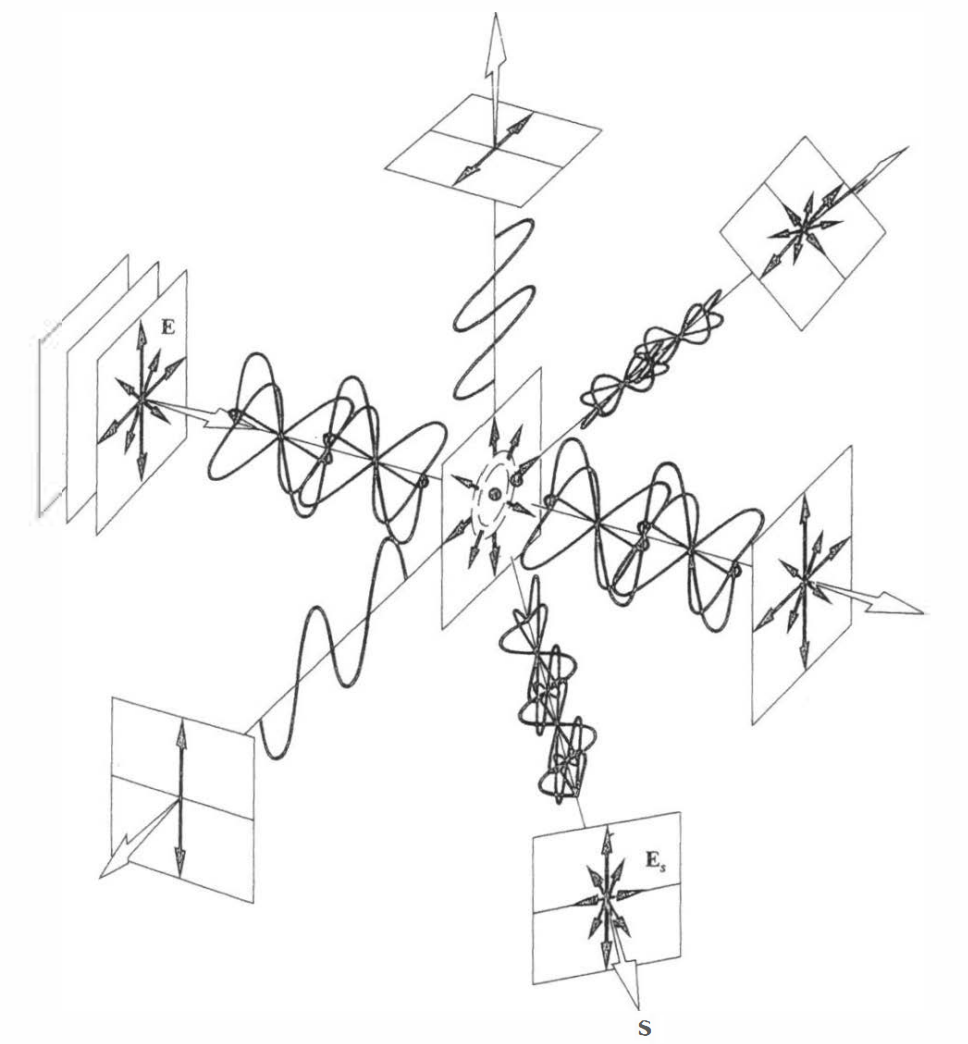
\includegraphics[scale=0.5]{scattering.png}
    \caption{Scattering of unpolarised light by a molecule.}
    \label{fig:scatter}
\end{figure}

The scattering mechanism of light on a molecule results from 
the electric-dipole radiation from the now energised molecule.
The direction of oscillation of the dipole will be aligned with 
the direction of linearly polarised light. Due to the pattern 
of electric field found from an oscillating electric dipole, an 
example of which can be found in Figure \ref{fig:dipole}below

\begin{figure}[H]
    \centering
    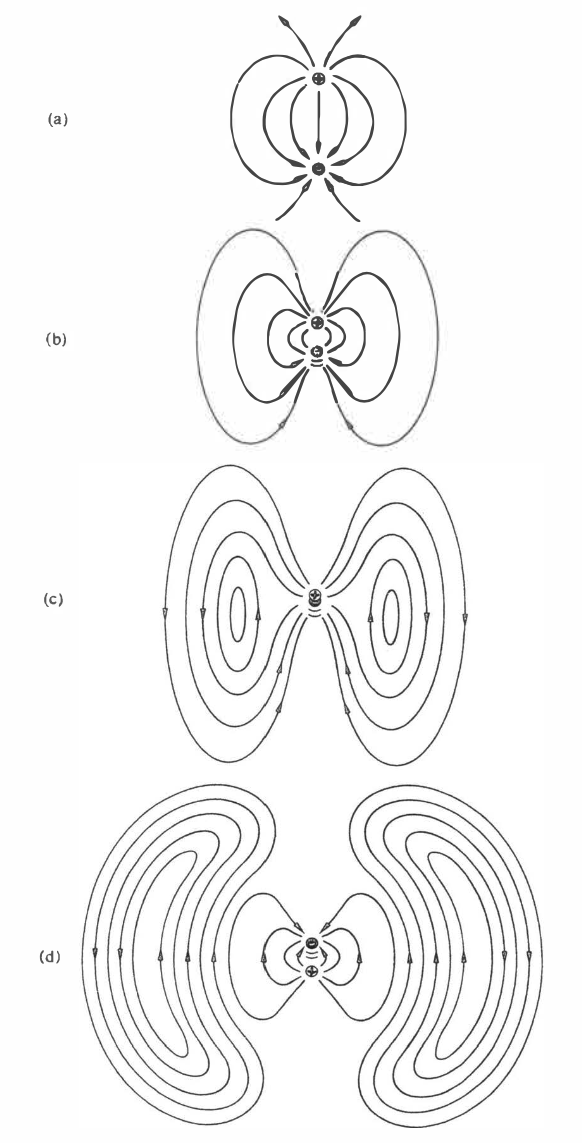
\includegraphics[scale=0.5]{efiled.png}
    \caption{Scattering of unpolarised light by a molecule.}
    \label{fig:dipole}
\end{figure}

It is important to note that the dipole will not radiate in the 
direction of oscillation.

In liquids, the spatial distribution of the molecules will 
impact the scattering of light. Because of the forces between 
the molecules and the fact that the molecules are spaced out 
more regularly, scattering of molecules in any other direction 
than forward tends to be quite weak.

Polarised light can also be replicated using polarisers 
and analysers. Law of Malus states that the intensity 
transmitted by the analyser varies as the square of the 
cosine of the angle between the analyser and polariser.

Unpolarised light incident on a dielectric material like glass 
will produce a transmitted or refracted ray as well as a 
reflected ray as seen in Figure \ref{fig:brewsters} below.

\begin{figure}[H]
    \centering
    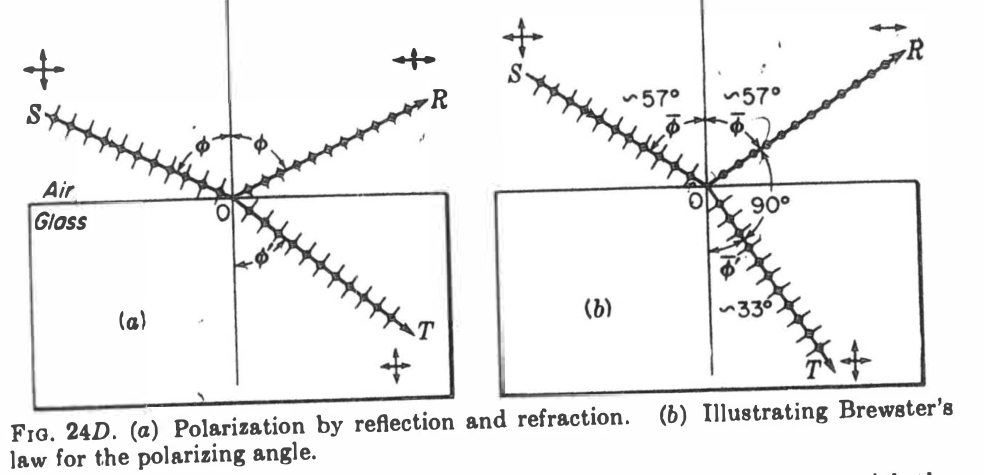
\includegraphics[scale=0.2]{brewsters.png}
    \caption{Scattering of unpolarised light by a molecule.}
    \label{fig:brewsters}
\end{figure}

As the angle of incidence approaches a special angle, dubbed 
the Brewster's angle, the polarisation of the reflected light 
approaches linearly polarised in one direction and the angle 
between the reflected light and the refracted light becomes 
a right angle. The reflected light being maximally polarised
in the plane perpendicular to the plane of incidence 
arises due to the fact that as the incident light sets the 
electrons in the atoms of the glass into oscillation, the 
reradiation generates the reflected beam. Thus it becomes 
polarised in one direction as the oscillating dipoles will 
only radiate in that direction.

In glass, at a normal incidence, the reflected intensity of 
light will be 4 per cent its total intensity, so 96 per cent 
of it is transmitted. This will be useful when we calculate 
the intensities to verify Fresnel's equations. For polarised 
light perpendicular to the plane of the incidence, subscripted
$s$, the corresponding Fresnel equation is,

\begin{equation}
    \frac{R_s}{E_s} = \frac{\sin{(\phi - \phi ')}}{\sin{(\phi 
    + \phi ')}}.
\end{equation}

Similarly, for polarised light parallel to the plane of incidence,
subscripted $p$,

\begin{equation}
    \frac{R_p}{E_p} = \frac{\tan{(\phi - \phi ')}}{\tan{(\phi 
    + \phi ')}}.
\end{equation}

Geometrically we can define an azimuthal angle, $\psi$, so that
\begin{equation}
    \tan{\psi} = \frac{R_p}{R_s}.
\end{equation}

At small angles, we can set the sines equal to the tangents and 
so $\frac{R_s}{E_s}\approx \frac{R_p}{E_p} = \frac{R}{E}$. We can 
then define $R_{12} = \frac{R^2}{E^2}$.

For metals, another constant, k, that describes the absorption of
light as it enters the metal must be used. This is because metals 
contain many free electrons. We can now define two general equations 
for any material, dielectric and metal.

\begin{equation} \label{eq:reflection}
    R_{12} = \frac{(1-n)^2+k^2}{(1+n)^2+k^2}.
\end{equation}

The associated phase delay is then,

\begin{equation} \label{eq:phi}
    \phi = \arctan{\left(\frac{2k}{1-n^2-k^2}\right)}.
\end{equation}



\section{Experimental Setup}
For the experiments explored in this report, the general 
setup is shown in the diagram below in Figure \ref{fig:diagram}.

\begin{figure}[H]
    \centering
    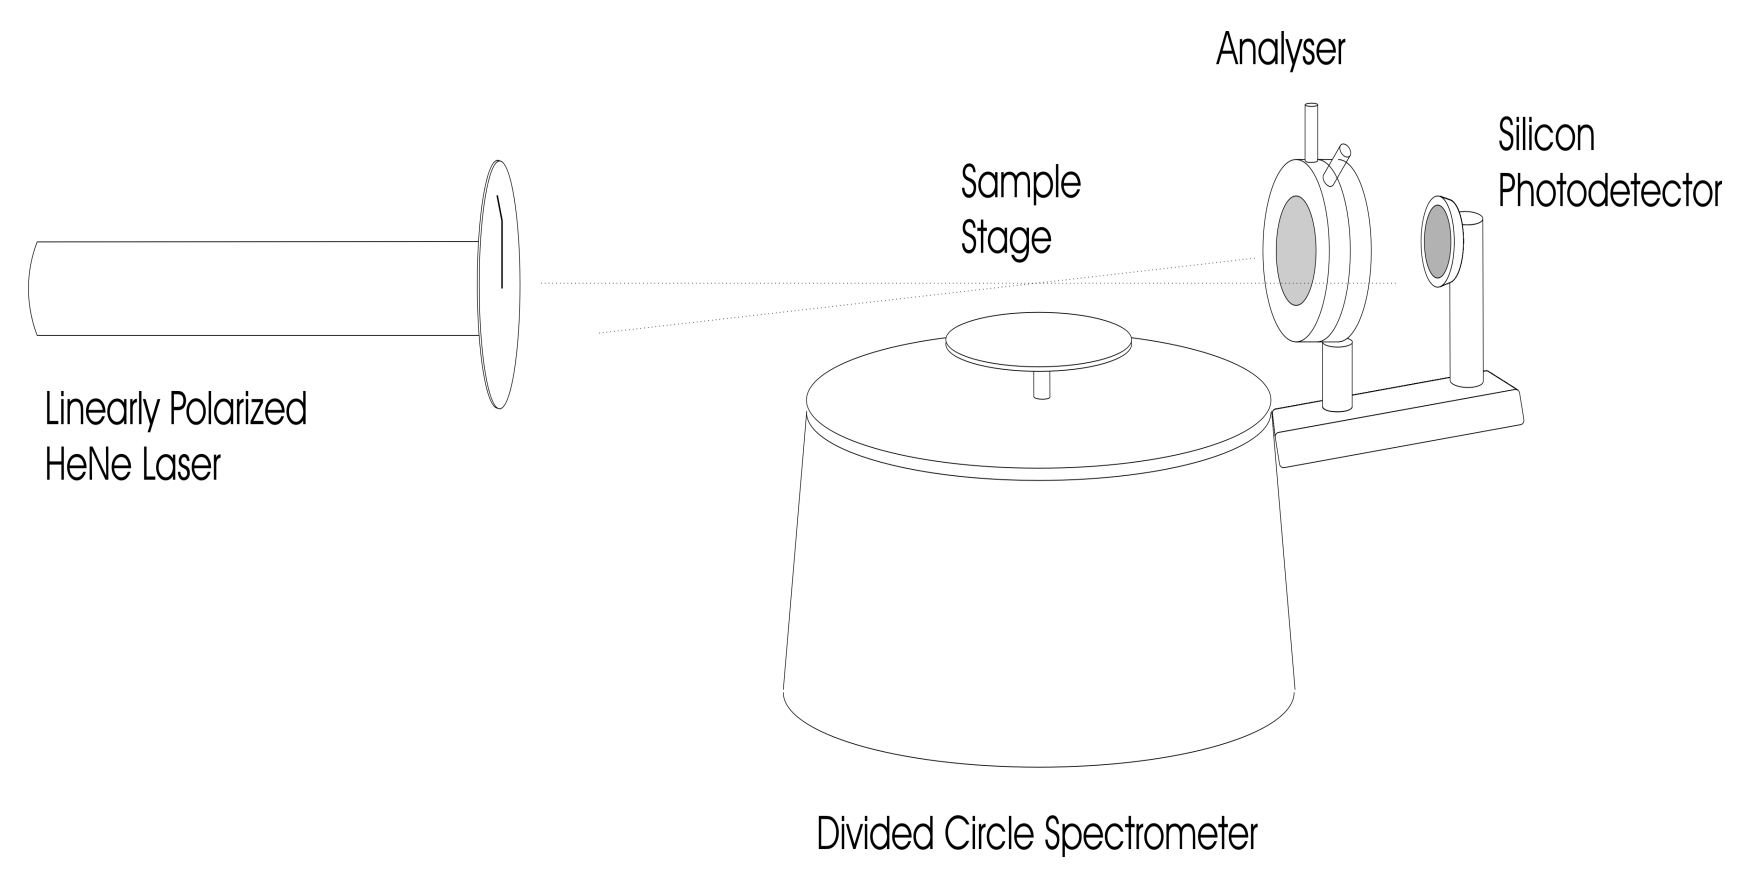
\includegraphics[width=0.8\textwidth]{experimentsetup.png}
    \caption{Schematic drawing of a basic experimental layout}
    \label{fig:diagram}
\end{figure}

By using a linear polariser filter, we measure the angle, $\theta^\circ$,
for which the polariser infront of the laser makes to make the light 
vertically polarised is $199 \pm 0.5 ^\circ$. Likewise, the horizontal angle is 
$244 \pm 0.5^\circ$. Throughout the report, we will take the azimuthal angle, $\phi$, 
to be the angle that is read off the spectrometer with an absolute uncertainty of 
$\pm 0.25^\circ$.

\section{Part I}
\subsection{Experiment 1: Scattering}
\subsubsection{Method}
In this first experiment, we placed solutions of Ajax and Dettol 
on the circle spectrometer. With the laser pointed at the solution,
illuminating the liquid and then scattering light around the bottle,
we moved the photodetector around the circle spectrometer, measuring 
the intensity of light at 3 different angles to the laser emitter, 
i.e parallel, $45^\circ$ to and perpendicular to the 
emitter. 

The detector was then kept 90 degrees to the beam. The half wave plate 
was aligned to begin recording data from a horizontal starting orientation.
The analyser in front of the detector was set to produce a maximum reading 
of intensity.

We then further tested the orientation of scattered light by comparing 
horizontally and vertically polarised light incident on Dettol and Ajax 
particles. By placing the solution on the spectrometer and aligned the 
vertically polarised laser into the beaker. The detector was then spun
around the spectrometer arm to capture the intensity of light at different 
azimuthal angle, $\phi$. 


\subsubsection{Results}
The tentative results are shown in the table below in Figure \ref{tab:table}.

\begin{table}[htbp]
    \centering
      \begin{tabular}{|c|c|c|}
      Angle/Intensity & Ajax ($\mu A$) & Dettol ($\mu A$) \\
      \hline
      Parallel & 0.398 & 0.463 \\
      $45^\circ$ & 0.18  & 0.435 \\
      Perpendicular & 0.026 & 0.304 \\
      \end{tabular}
    \caption{Table displays the relationship between the angle 
    observed and the intensity of the scattering. It is important
    to note that the intensity falls as the angle increases but due 
    to low sample of points, hard to describe proper trendline.}
    \label{tab:table}
\end{table}

\begin{figure} [H]
    \centering
    \scalebox{0.75}{\input{horizontaldettol.pgf}}
    \label{fig:horizontaldettol}
    \caption{Hysteresis Loop found experimentally for I = 1.6A.}
\end{figure}

\begin{figure} [H]
    \centering
    \scalebox{0.75}{\input{verticaldettol.pgf}}
    \label{fig:verticaldettol}
    \caption{Hysteresis Loop found experimentally for I = 1.6A.}
\end{figure}

\subsubsection{Analysis}

\subsection{Experiment 2: Linear Polarisation}
\subsubsection{Method}
In this second experiment, we want to verify Malus' law. We will do 
this by keeping the vertical analyser upright and changing angle of 
the polariser on the laser. In this setup, the analyser and photodiode
is parallel to the laser.

Using Jones' vector notation, we can represent the transmission of 
light through the polariser and analyser as matrix states. Polarisation
is represented by a 2 by 1 Jones vector, since we are dealing with linear 
polarisation, we assume the phase of the orthogonal components to be equal,

\begin{equation}
    \textbf{J} = \begin{pmatrix}
        E_{0x} \\ 
        E_{0y}
    \end{pmatrix}.
\end{equation}

The initial polarisation on the laser is vertically orientated 
so we can represent this using the Jones vector,

\begin{equation}
    \textbf{y} = \begin{pmatrix}
        0 \\
        1
    \end{pmatrix}.
\end{equation}

Or more specifically,

\begin{equation} \label{eq:J}
    \textbf{J} =\begin{pmatrix}
        0 \\
        E_{oy}
    \end{pmatrix}.
\end{equation}

To find the Jones' matrix representation of an analyser at some angle 
$\theta$ to the plane of polarisation of the incoming light, we first 
consider some arbitrary reference frame for which the polariser is 
aligned with, at an angle $\theta$. So we have to introduce a rotation
matrix with angle $\theta$ to transform the coordinates into the reference 
frame of the polariser,

\begin{equation}
    \textbf{$R_+$} = \begin{pmatrix}
        \cos{\theta} & \sin{\theta} \\
        -\sin{\theta} & \cos{\theta}
    \end{pmatrix}.
\end{equation}

We can now just apply the follow Jones matrix to remove any orthogonal 
components,

\begin{equation}
    \textbf{$P_y$} = \begin{pmatrix}
        0 & 0 \\
        0 & 1
    \end{pmatrix}.
\end{equation}

Now we can transform the coordinates back into the reference frame of 
the lab by applying the rotation matrix again but with $-\theta$,

\begin{equation}
    \textbf{$R_-$} = \begin{pmatrix}
        \cos{-\theta} & -\sin{\theta} \\
        \sin{\theta} & \cos{\theta}
    \end{pmatrix}.
\end{equation}

Putting all of this together,

\begin{equation}
    \textbf{J'} = R_- P_y R_+ \textbf{J}.
\end{equation}

Computing the matrix multiplication will result in,

\begin{equation}
    \textbf{J'} = \begin{pmatrix}
        \sin^2{\theta} & -\cos{\theta}\sin{\theta} \\
        -\cos{\theta}\sin{\theta} & \cos^2{\theta}
    \end{pmatrix} \textbf{J}.
\end{equation}

Substituting in Equation \ref{eq:J}, we find,
\begin{align}
    \textbf{J'} &= \begin{pmatrix}
        \sin^2{\theta} & -\cos{\theta}\sin{\theta} \\
        -\cos{\theta}\sin{\theta} & \cos^2{\theta}^2
    \end{pmatrix} 
    \begin{pmatrix}
        0 \\
        E_{0y}
    \end{pmatrix} \\
    &= E_{0y}\begin{pmatrix}
        \cos{\theta}\sin{\theta} \\
        \cos^2{\theta}
    \end{pmatrix}
\end{align}

Taking the magnitude of the Jones vector to represent its magnitude,

\begin{equation}
    I = |\textbf{J'}|^2 = E_{0y}(\sin^2{\theta}\cos^2{\theta}+\cos^4{\theta}).
\end{equation}

Simplifying the equation and then replacing $E_{0y}$ with $I_0$,

\begin{align}
    I &= I_0(\cos^2{\theta}(1-\cos^2{\theta})+\cos^4{\theta}) \\
    &= I_0\cos^2{\theta}.
\end{align}

We recover Malus' law.

\subsubsection{Results}
\begin{figure} [H]
    \centering
    \scalebox{0.75}{\input{maluslaw.pgf}}
    \label{fig:ml}
    \caption{Hysteresis Loop found experimentally for I = 1.6A.}
\end{figure}
\subsubsection{Analysis}

\subsection{Experiment 3: Circular Polarisation}
\subsubsection{Method}
In this third experiment, the same setup from Experiment 2 is used 
except that the analyser is replaced with a filter of either quarter 
wave plate or circular polariser.

Using Jones' vector notation we find the matrix associated with quarter 
wave plates to be,

\begin{equation}
    \textbf{P}_{quarter} = e^{\frac{i\pi}{4}}\begin{pmatrix}
        1 & 0 \\
        0 & -i
    \end{pmatrix}
\end{equation}

assuming the fast axis is the vertical axis in this case, i.e $E_y$ leads 
$E_x$. 

\subsubsection{Results}
\begin{figure} [H]
    \centering
    \scalebox{0.75}{\input{quarter_waveplate.pgf}}
    \label{fig:quarter_wave}
    \caption{Hysteresis Loop found experimentally for I = 1.6A.}
\end{figure}

\begin{figure} [H]
    \centering
    \scalebox{0.75}{\input{circ.pgf}}
    \label{fig:circ}
    \caption{Hysteresis Loop found experimentally for I = 1.6A.}
\end{figure}
\subsubsection{Analysis}

\section{Part II}
\subsection{Experiment 1: Reflection from Dielectrics}
In these experiments we want to determine the optical constants, n,
and k for the glass prism.

\subsubsection{Method}
Firstly, we need to determine Brewster's angle for the glass prism in 
order to determine its refractive index. Brewster's angle is related 
to the refractive index, n, through the following formula,

\begin{equation}
    \tan{\theta_{B}} = n.
\end{equation}

A prism is now mounted on the spectrometer table with its reflecting 
face directed towards the laser to produce a normal incidence. Rotating 
the table to produce an angle of incidence of 45 degrees to the normal we 
can now find the reflected beam visible as a spot on the screen on the 
spectrometer arm. By rotating the half-wave plate infront of the laser, 
and the table we can begin search for Brewster's angle.

We know that at Brewster's angle, the reflected light will be maximally
polarised in the direction perpendicular to the plane of incidence. This 
will correspond to a minimum intensity on the screen.

Once Brewster's angle is found, we can determine the polarisation of the
laser.

Next, we will find the reflectance intensities, $R{p}$ and $R_{s}$. We 
know $E{s}$ and $E{p}$ by simply measuring the intensity of horizontally 
and vertically polarised light without any reflection. Therefore we can 
find the reflectance coefficient, which we expect to be 0.04 at the normal 
incidence.

In Task C, we will explore the effect of angle of incidence on the 
polarisation of the reflected light. The polarisation of the reflected 
light parallel to the plane of incidence will flip when the angle changes 
past the critical angle i.e the angle at total internal reflection.

\subsubsection{Results}
\subsubsection{Analysis}
\subsection{Experiment 2: Reflection from Metals}
\subsubsection{Method}
We can find the optical constants n and k through using Equations 
\ref{eq:reflection} and \ref{eq:phi}. The half wave plate is rotated 
so that the polarised light is 45 degrees to the vertical. First, the 
table is adjusted so that the beam hits the mirror at 20 degrees to 
the normal. The spectrometer arm is moved to detect the reflected beam 
and the analyser is rotated such that a maximum intensity is achieved.

\subsubsection{Results}
\subsubsection{Analysis}
\newpage
\section{Appendix}
\subsection{Pre-Work Theoretical Questions}
\subsubsection{Question 2a}
\textbf{What is the condition for linearly polarised light to 
remain unaltered as it passes through a crystal?}

For the linearly polarised light to remain unaltered, the light 
incidence needs to experience no relative phase changes. Crystals
can either be isotropic or anisotropic. In the case of isotropic 
crystals, the linearly polarised light has to be pass through the 
crystal along its polarisation axis. Anisotropic materials have a 
property known as birefringence, where the crystal has a different
refractive index for each polarisation and propagation of light. 
The linearly polarised light must enter the crystal along the 
optical axis. This means that the light will only experience the
refractive index of ordinary rays. If light were to enter the crystal
in any other direction, then it would experience two refractive indexes
which will alter the polarisation of the wave. Similarly, in biaxial
crystals, there are two optical axes (binormals) that allow light to
travel through without birefringence.

\subsubsection{Question 2b}
\textbf{What are the conditions to create circularly polarised light?}

You can use a linear polariser to get linearly polarised light first
and then use a quarter wave layer to create a circular polariser. The 
corresponding phase difference needs to be 90 degrees. To achieve this,
the formula for phase difference in uniaxial crystals can be used,

\begin{equation}
    \Delta \phi = \frac{2\pi}{\lambda}(n_e-n_o)d.
\end{equation}
By adjusting the thickness, d, of the crystal appropriately as $n_e$ 
and $n_o$ are fixed, we can obtain a phase difference of 90 degrees. 
Then the quarter wave plate needs to placed at an angle of 45 degrees
with the plane of the incident polarised light.

\subsubsection{Question 2c}
\textbf{What is the effect of a quarter wave plate on circularly polarised light?}

The quarter wave plate will introduce a 90 degree phase shift which 
will convert circularly polarised light back to linearly polarised.

\subsubsection{Question 2d}
\textbf{What is the effect of a half wave plate on circularly polarised light?}

A half wave plate will introduce a phase difference of 180 degrees, 
meaning that the handedness of the circular polarisation will switch i.e 
right handed circular polarisation will turn into left handed circular
polarisation and vice versa.

\subsubsection{Question 2e}
\textbf{Sometimes the scattering of light off particles may lead to polarisation.
Explaining in terms of scattering, why is the sky blue and why clouds are grey?}

In 1871, Rayleigh discovered that when light is scattered by molecules or 
particles much smaller than the wavelength of the light, the intensity 
of the scattered light has the following property,

\begin{equation}
    I \propto \frac{1}{\lambda^4}.
\end{equation}

This is why the sky is blue as the lower wavelengths of light, i.e bluer, are 
scattered much more. At sunset, when the sun is low of the horizon, the blue
and violet light is scattered out of the direct line of sight, giving the sky
its redder tinge. In clouds, the particles are no longer small enough for 
Rayleigh scattering and instead we look at Mie scattering. Here we find that 
the droplets of water will scatter all wavelengths equally and so clouds are
perceived as white. As the clouds become thicker, more light is absorbed and 
less sunlight can penetrate, dimming the sky and the appearance of the cloud.

When light strikes a particle, it will induce an oscillation in the charges 
of the particle, causing it to re-emit light but they do so more strongly in
directions where the electric field is perpendicular to the direction of 
observation. For the original incoming light, it becomes polarised as the 
electric field in the direction of scattering is minimised.

\subsubsection{Question 2f}

\begin{figure}[H]
    \centering
    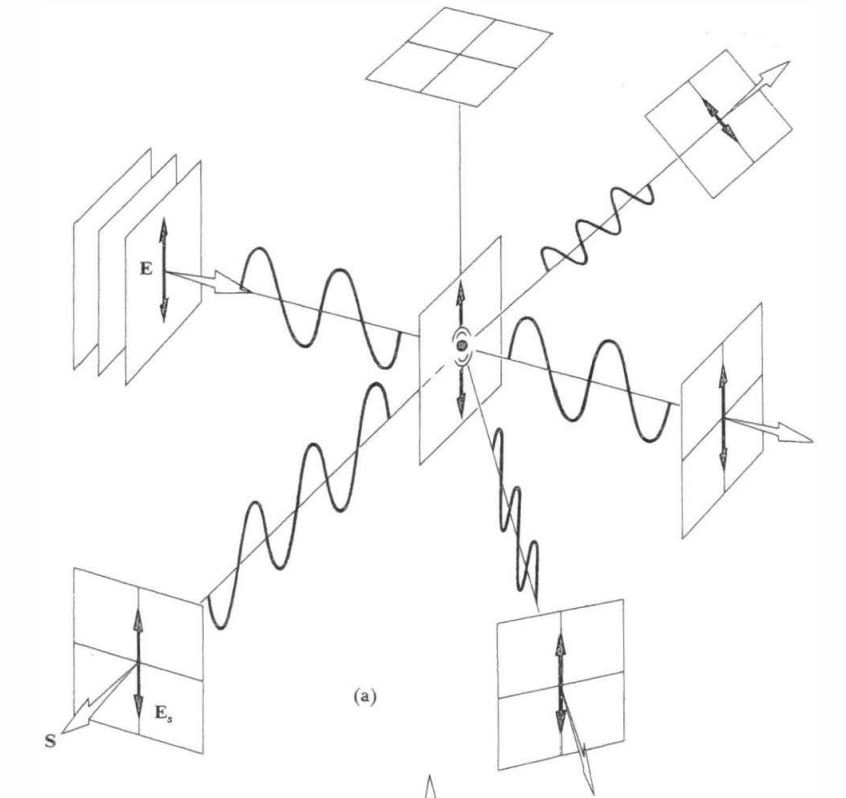
\includegraphics[width=0.8\textwidth]{prework.png}
    \caption{Scattering of polarised light by a molecule}
\end{figure}

Scattered light will only propagate in forward directions and not in the 
direction of the electric field. The magnitude will be equal in the 
directions orthogonal to the propagation of the electric field and decrease
as the angle between the propagation of the scattered wave and the propagation 
of the original wave's electric field is smaller.

\subsubsection{Question 2g}
Using
\begin{equation}
    I_1 = I_0 \cos^2{\theta}.
\end{equation}

a. 100\%
b. 50\%
c. 0\%
\subsection{Lab Book}
\subsubsection{Proper Attempt}

\begin{figure}[H]
    \centering
    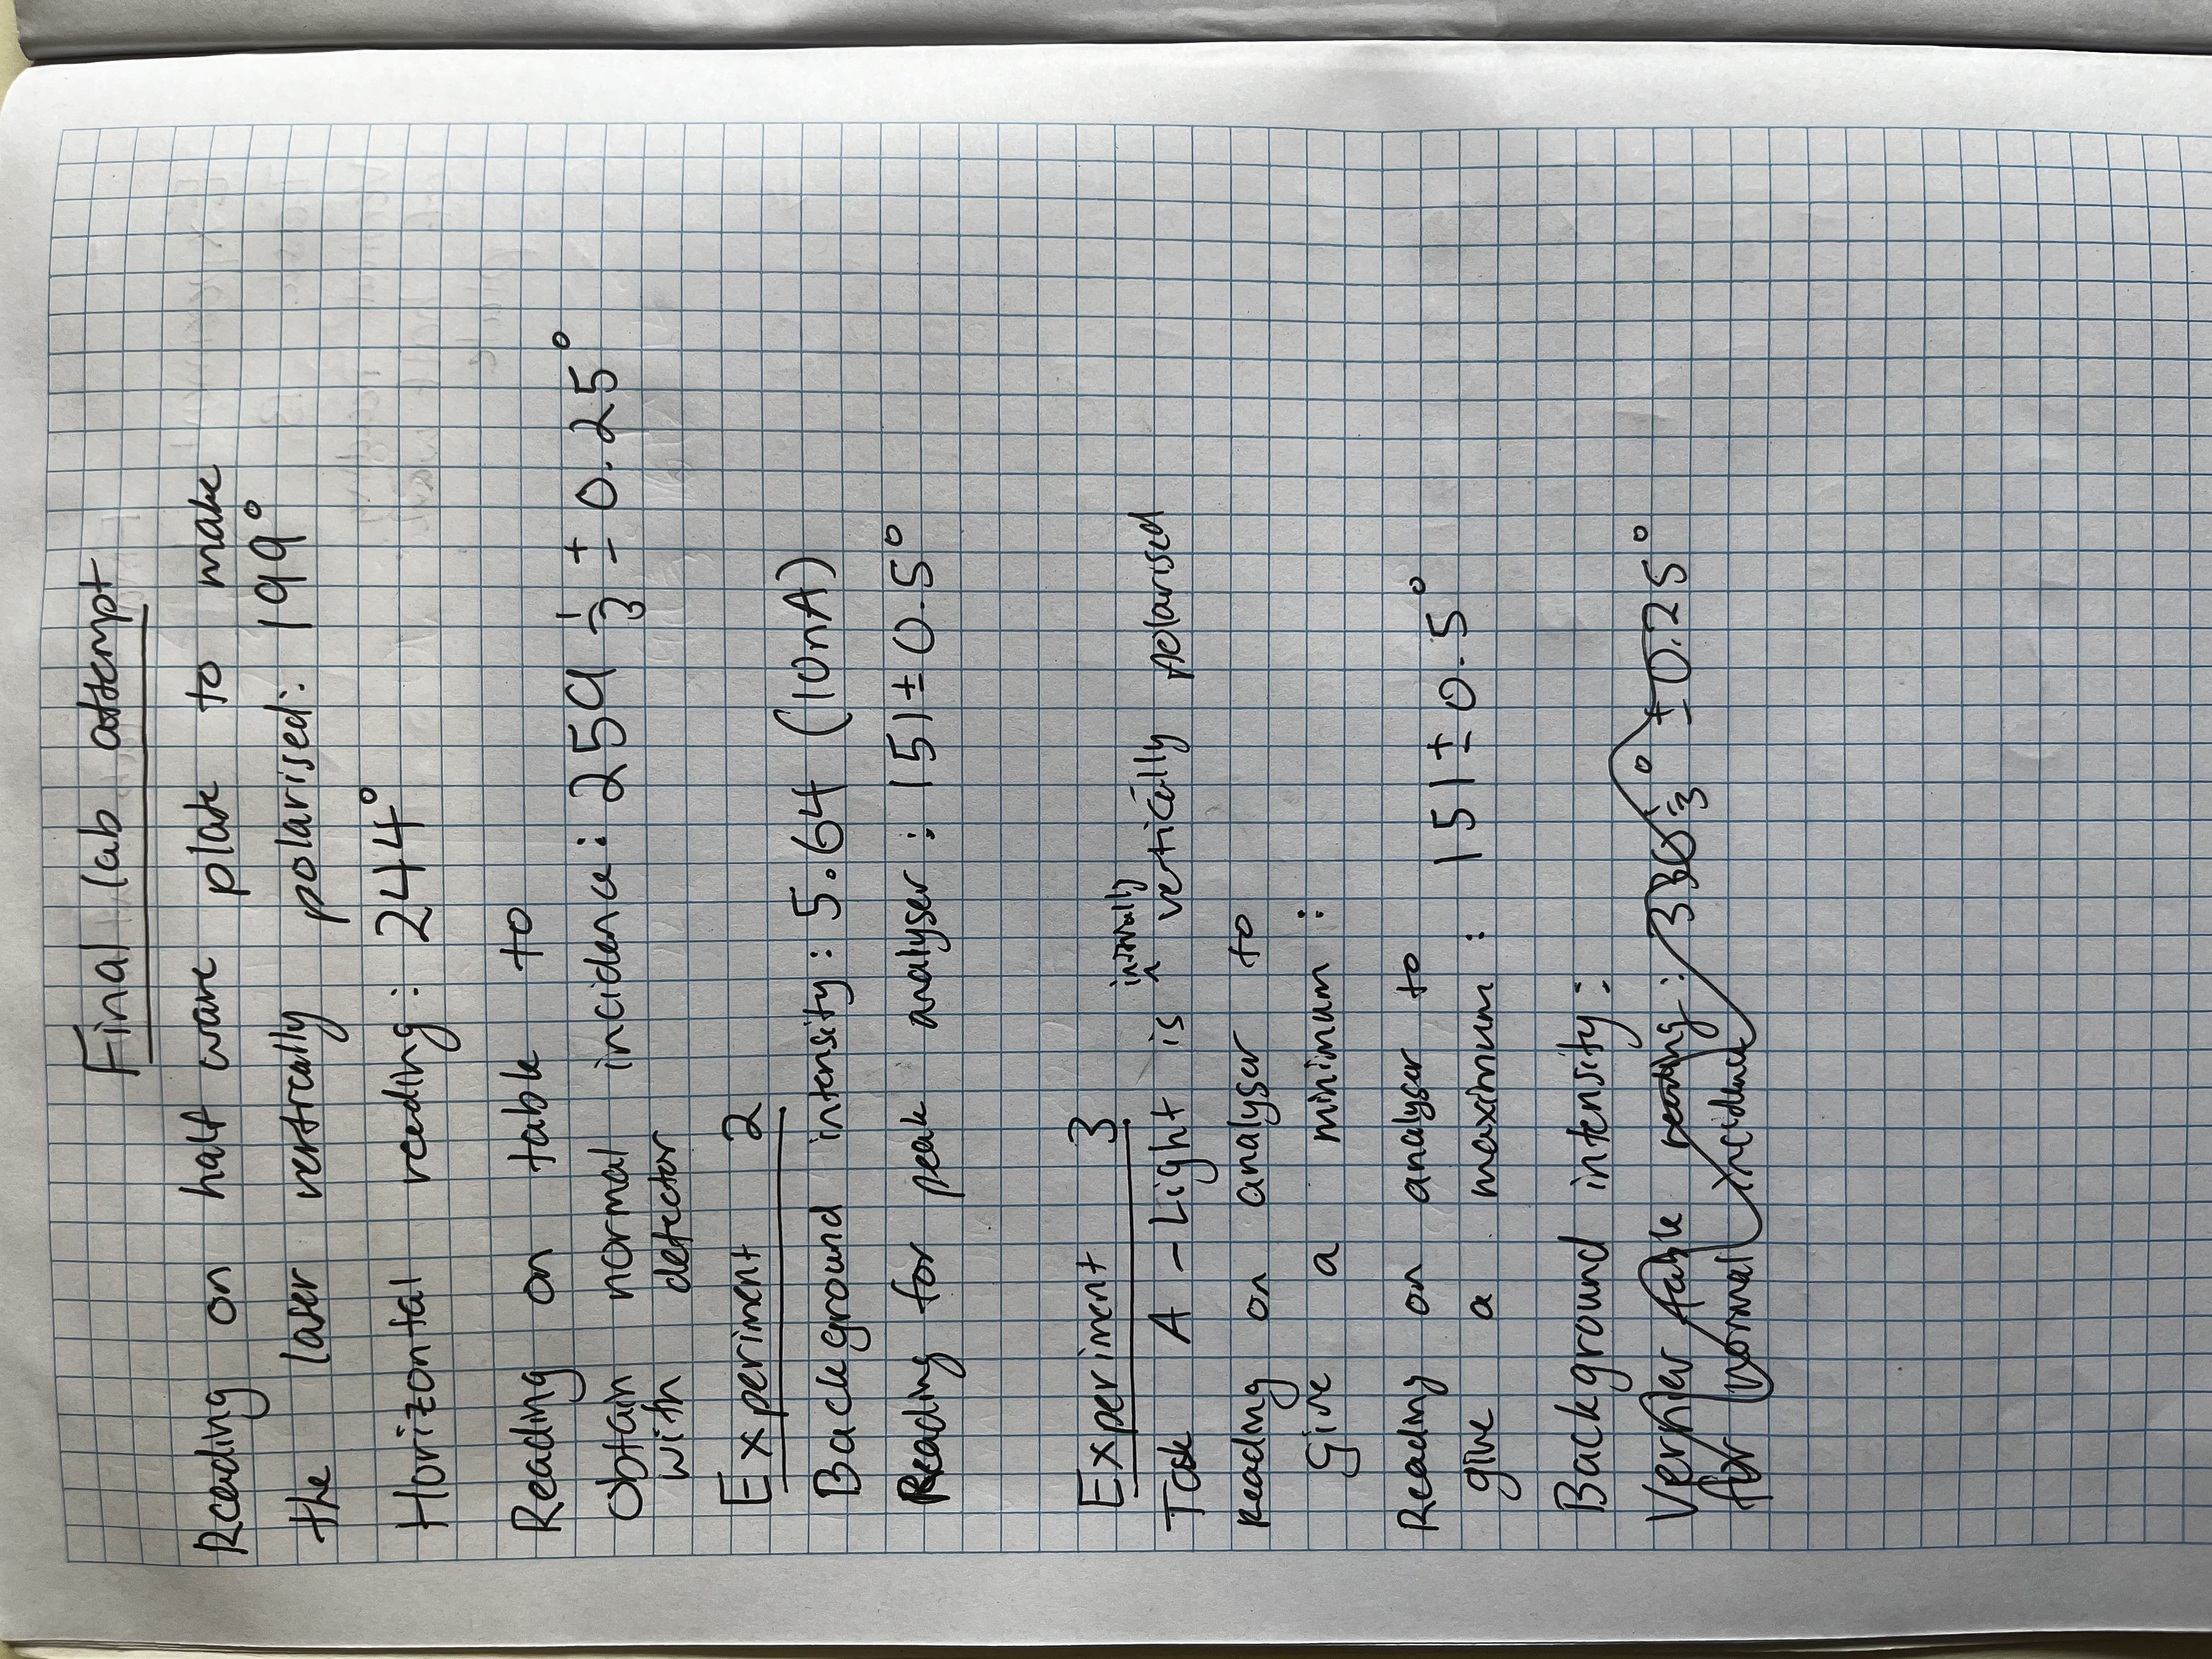
\includegraphics[width=0.8\textwidth,angle=270,origin=c]{labbook10.jpg}
\end{figure}

\begin{figure}[H]
    \centering
    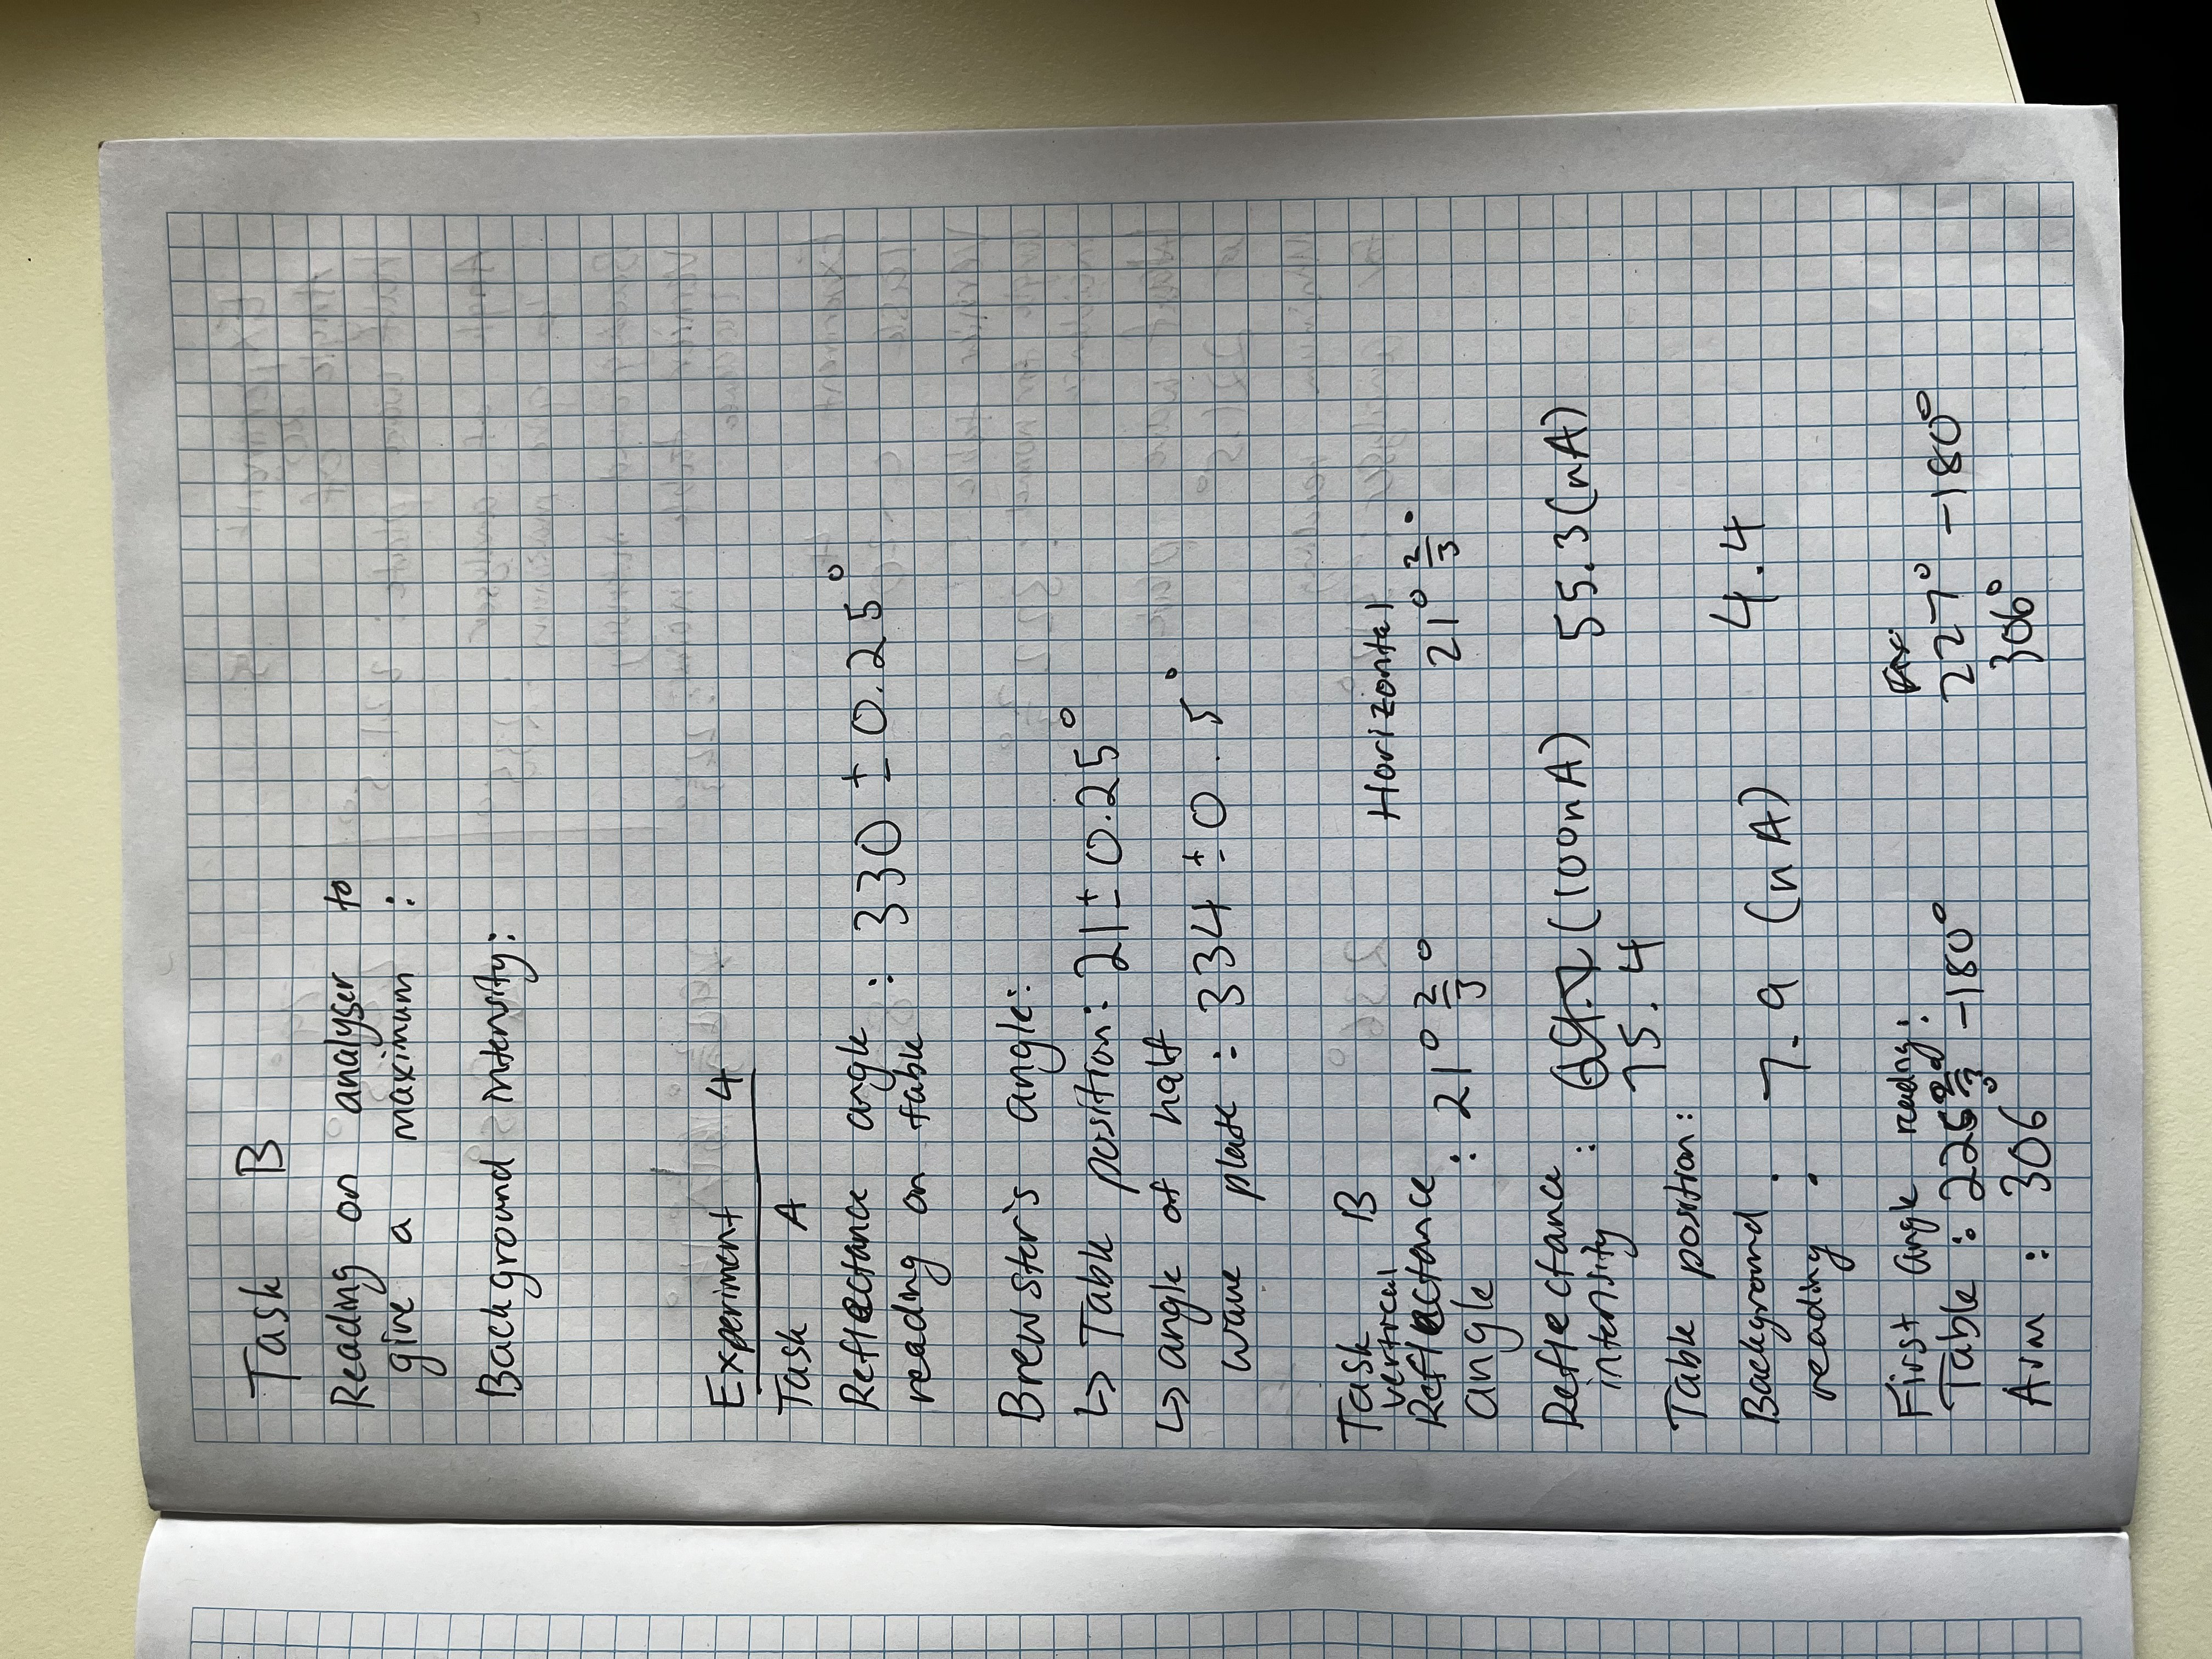
\includegraphics[width=0.8\textwidth,angle=270,origin=c]{labbook11.jpg}
\end{figure}

\begin{figure}[H]
    \centering
    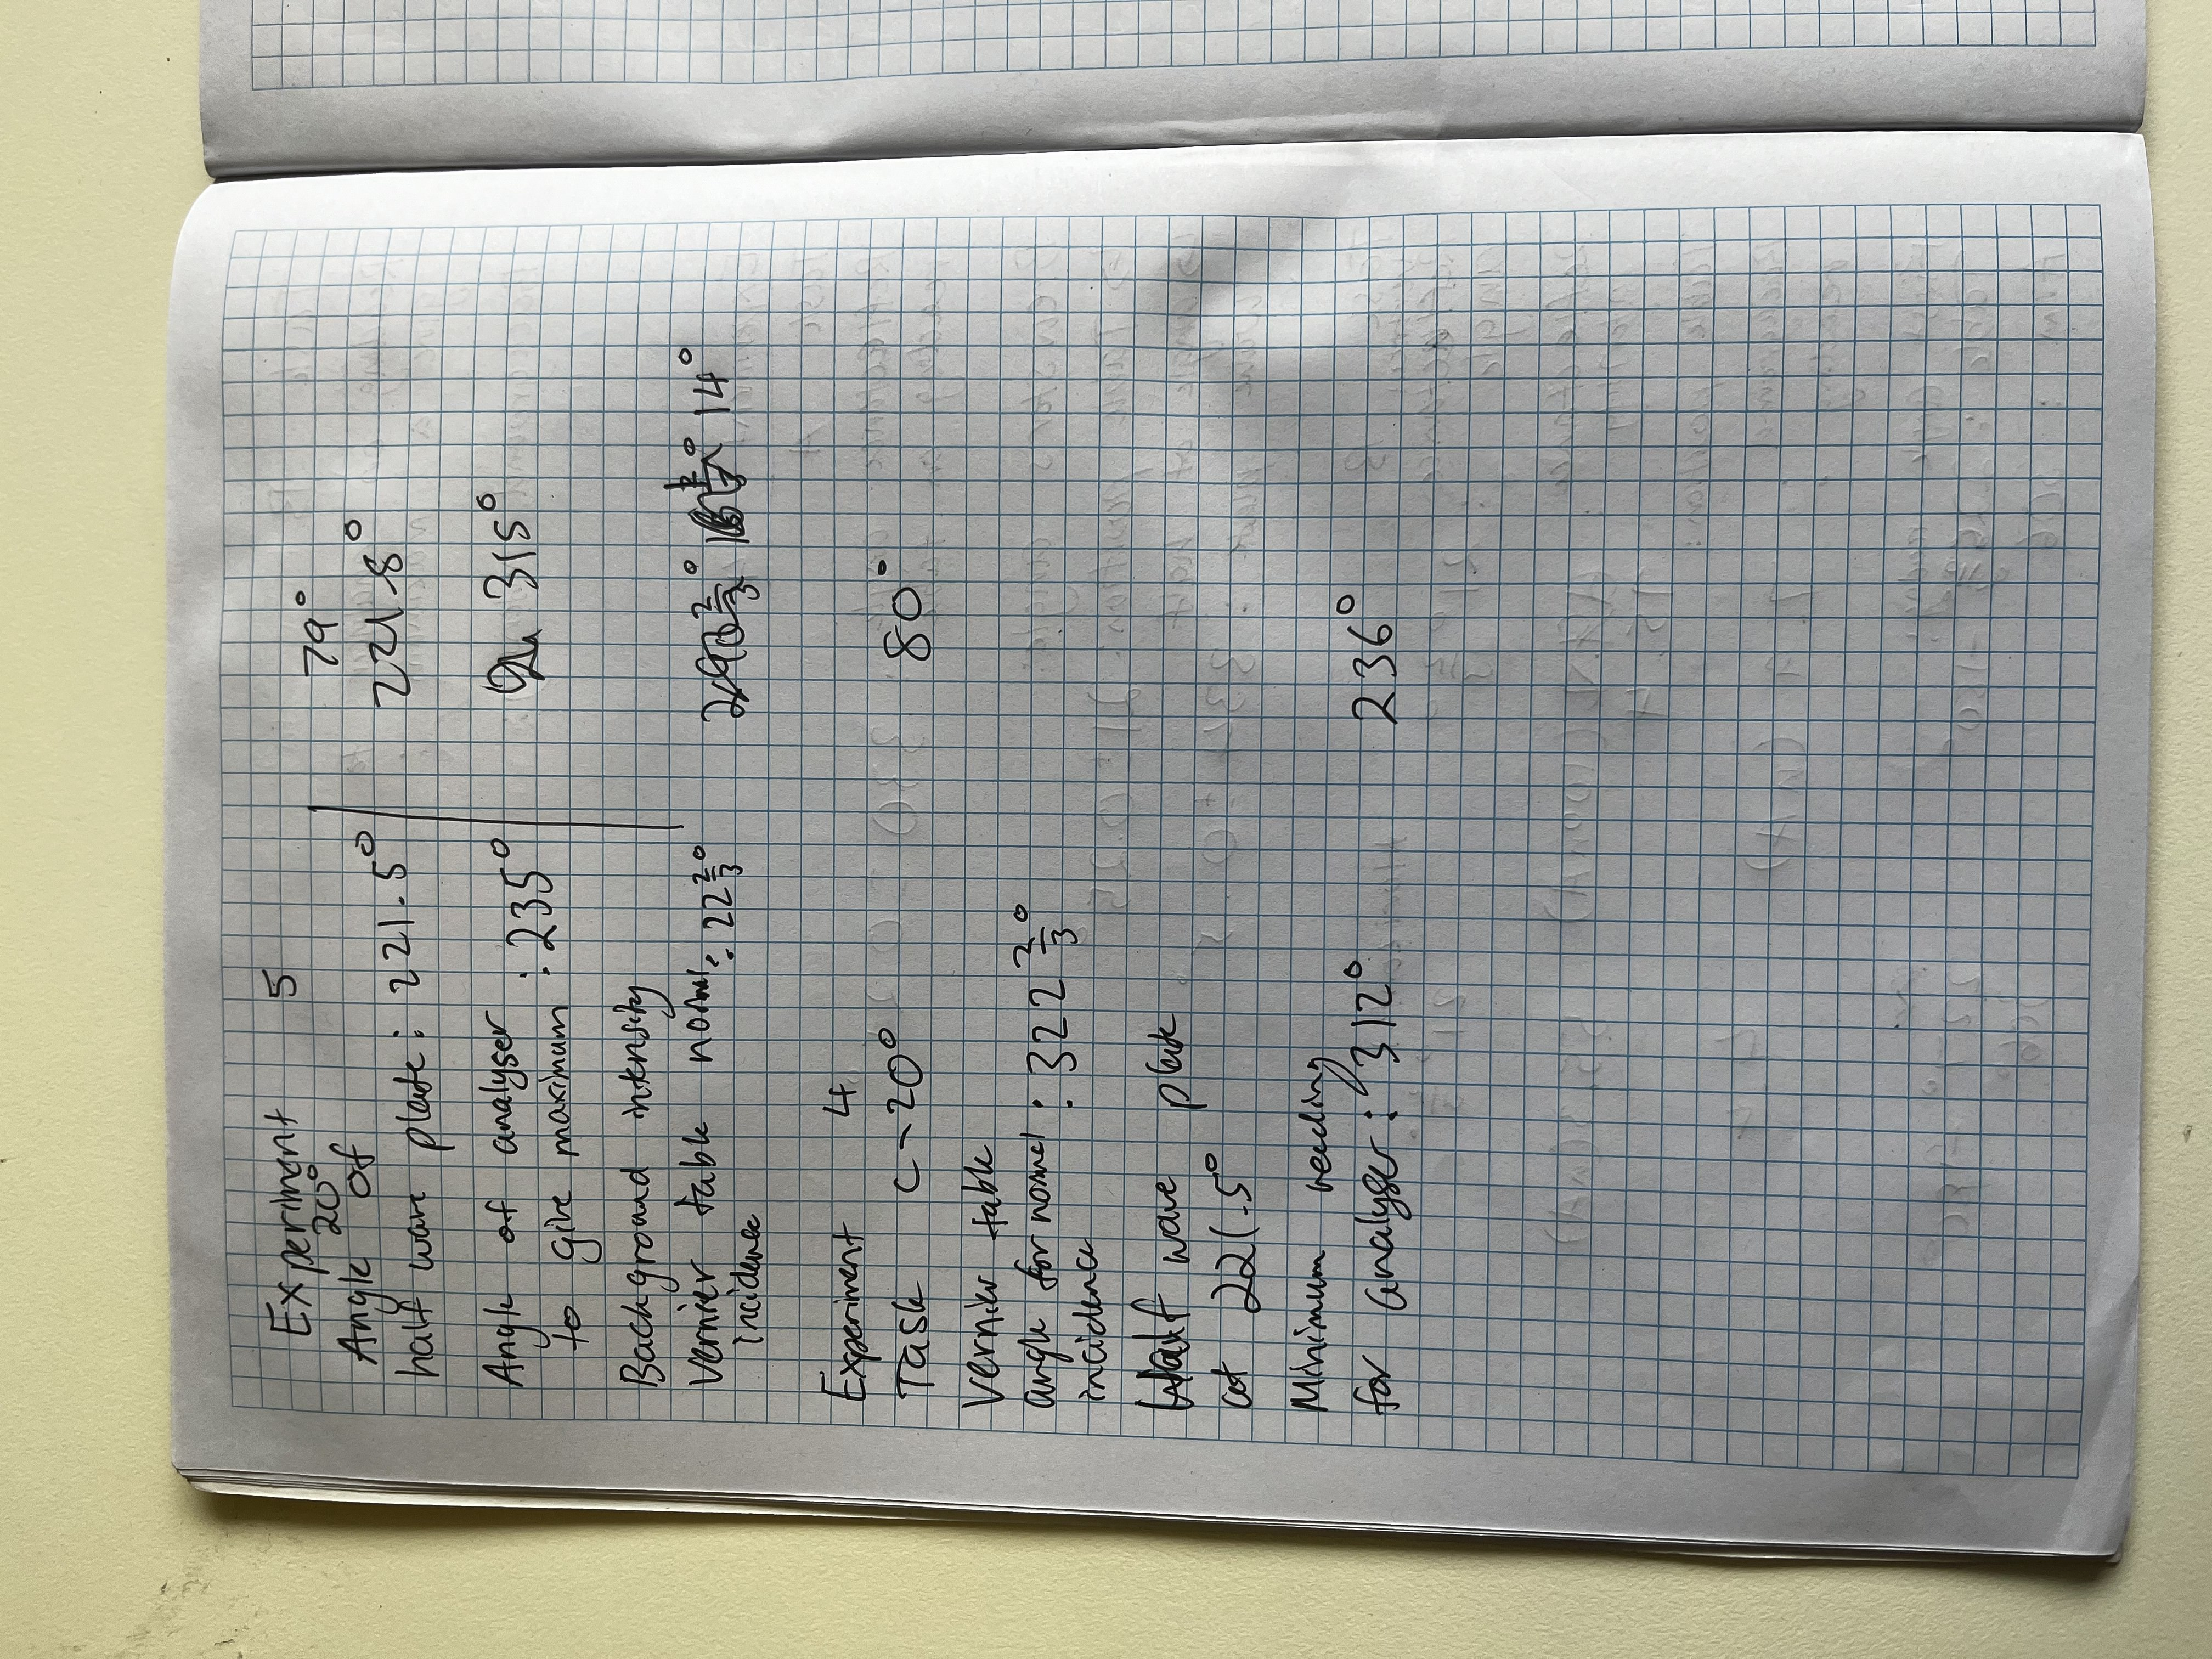
\includegraphics[width=0.8\textwidth,angle=270,origin=c]{labbook12.jpg}
\end{figure}


\subsection{Failed Attempts}
\begin{figure}[H]
    \centering
    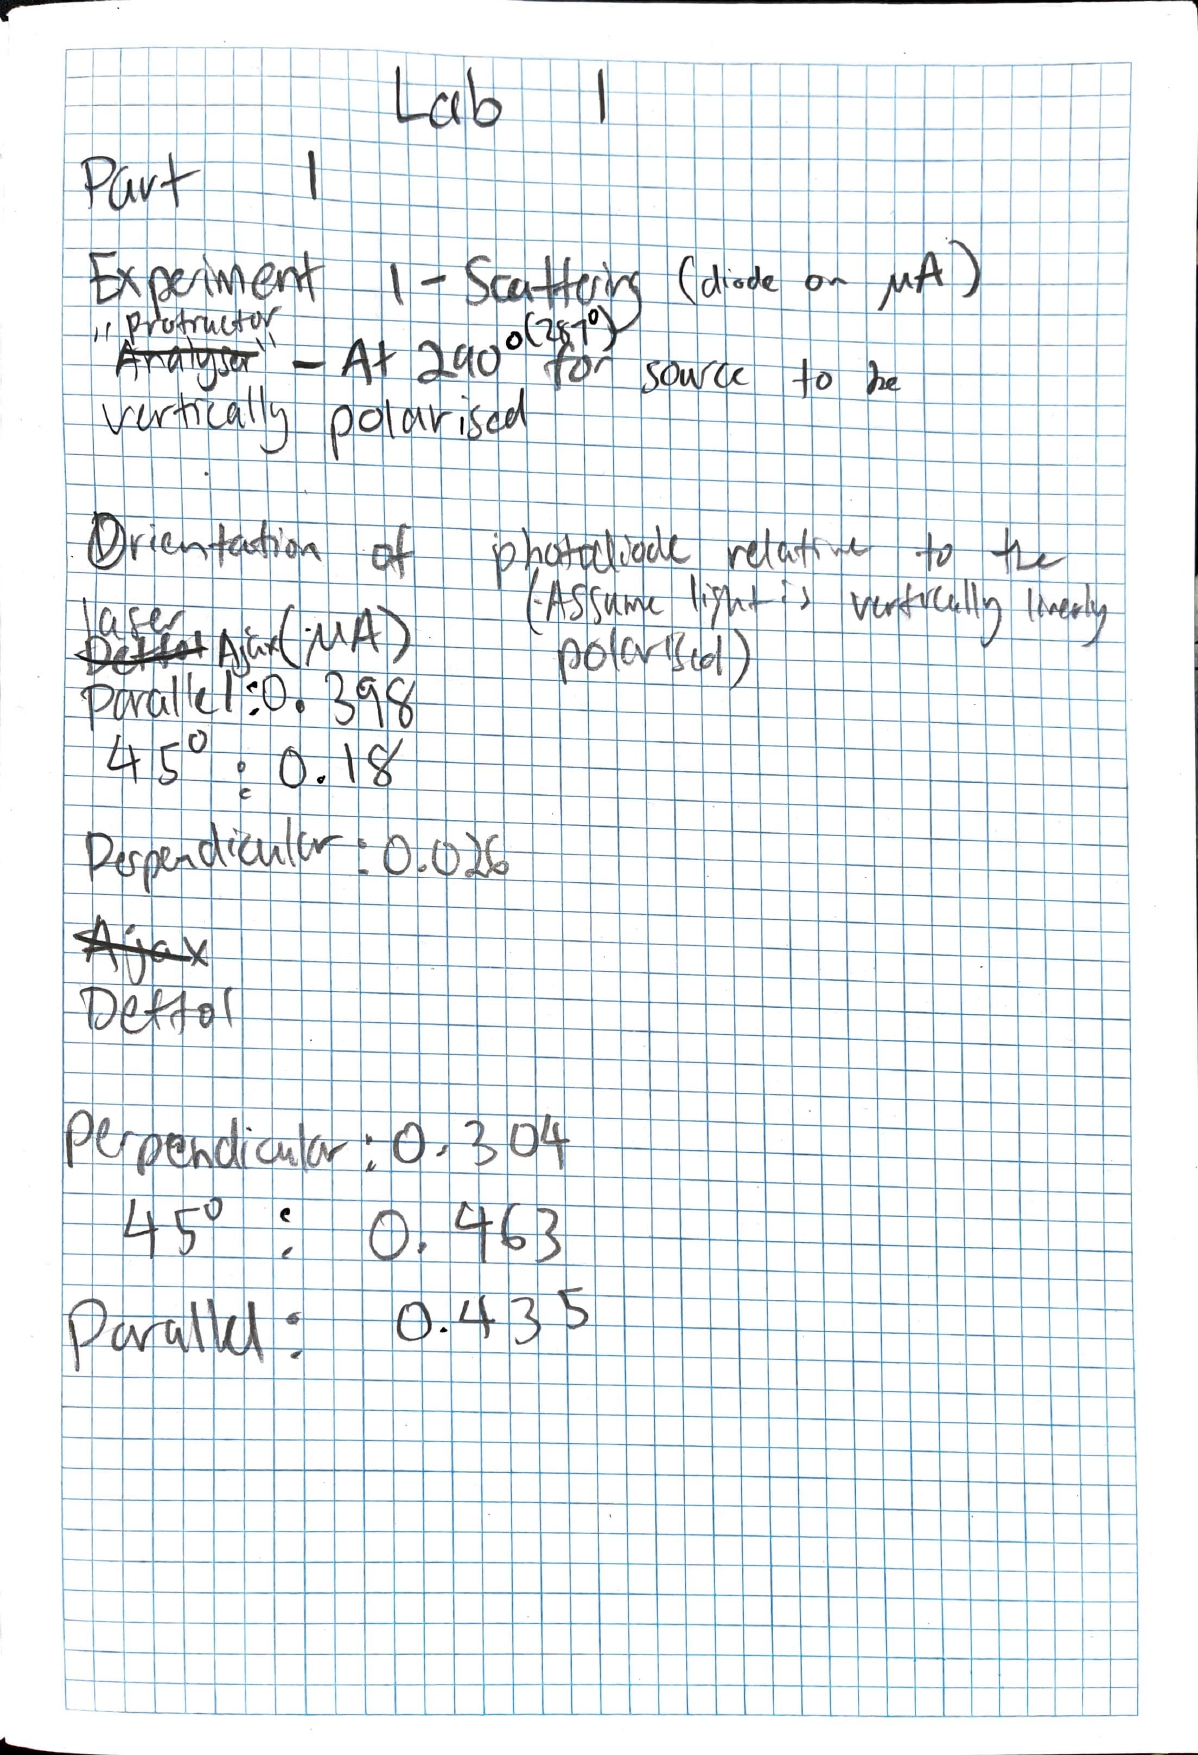
\includegraphics[width=0.8\textwidth]{labbook1.jpg}
\end{figure}

\begin{figure}[H]
    \centering
    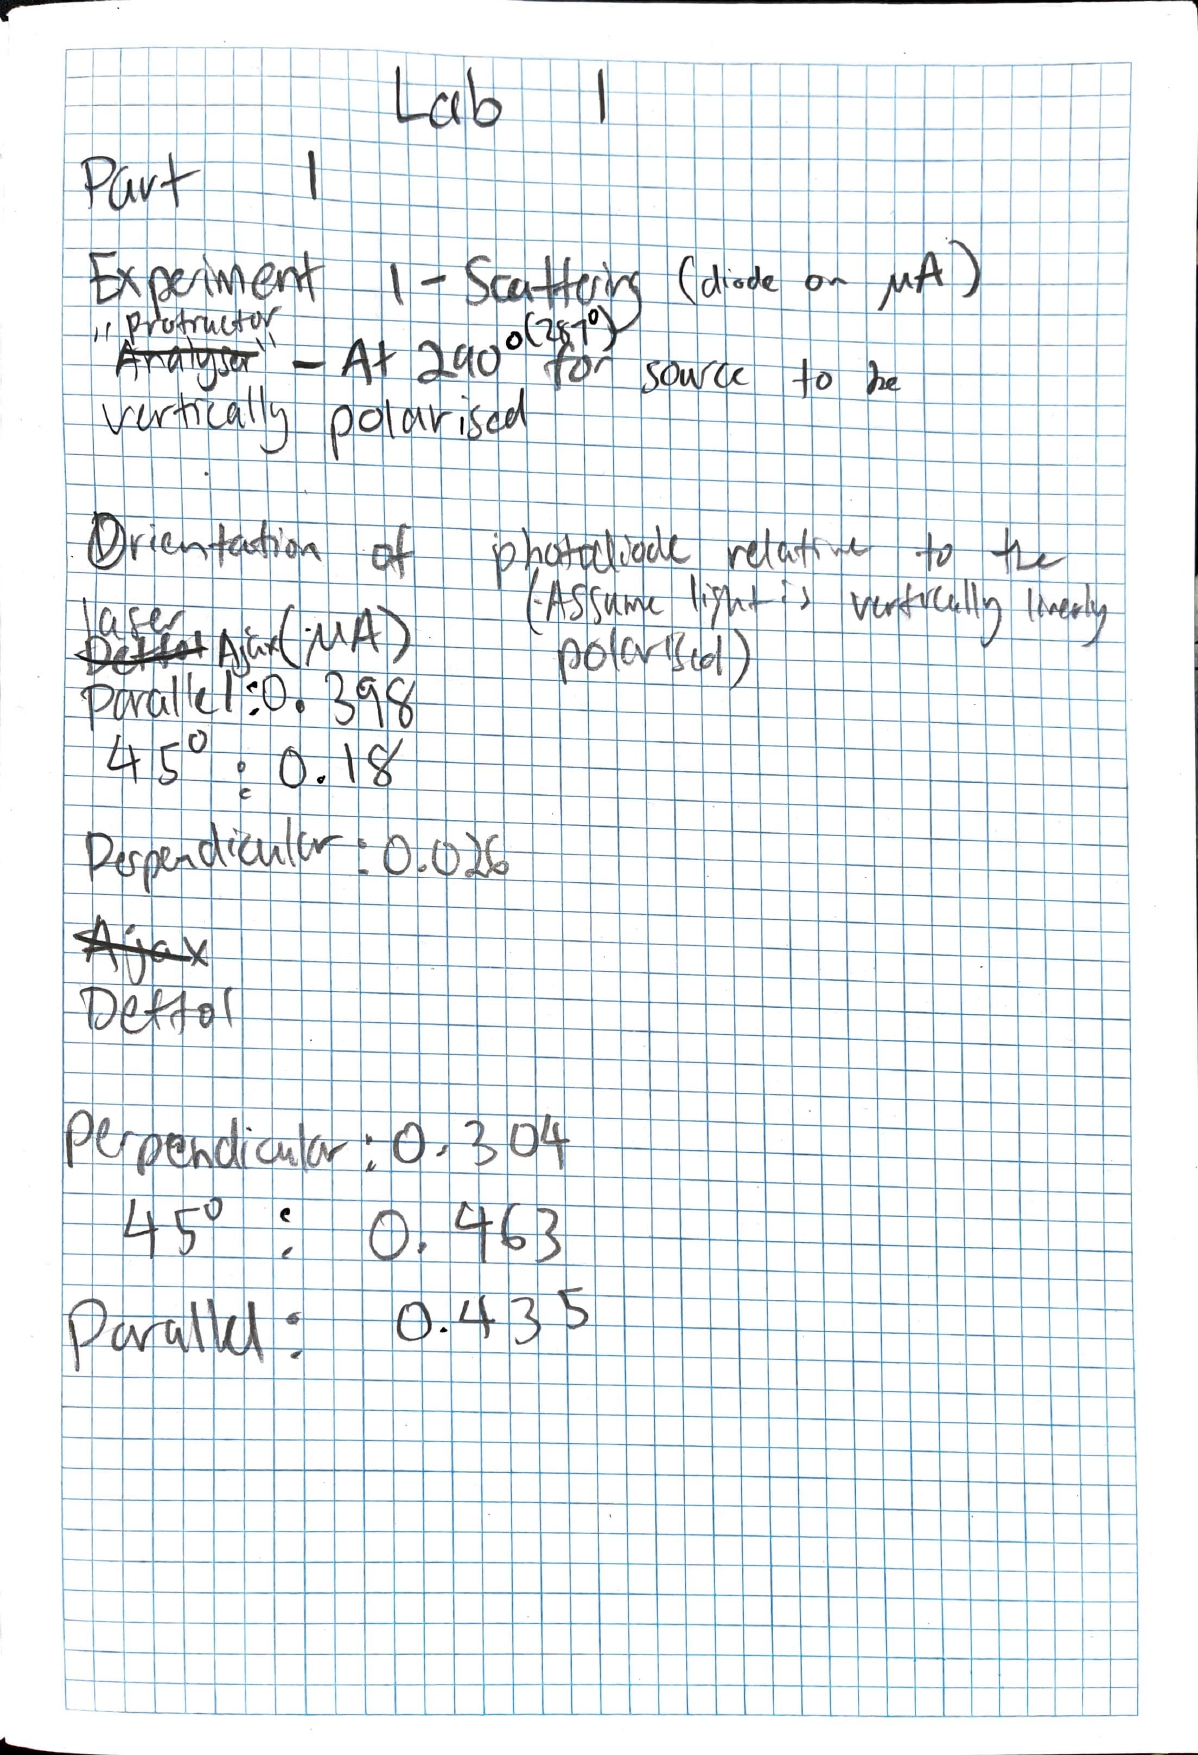
\includegraphics[width=0.8\textwidth]{labbook1.jpg}
\end{figure}

\begin{figure}[H]
    \centering
    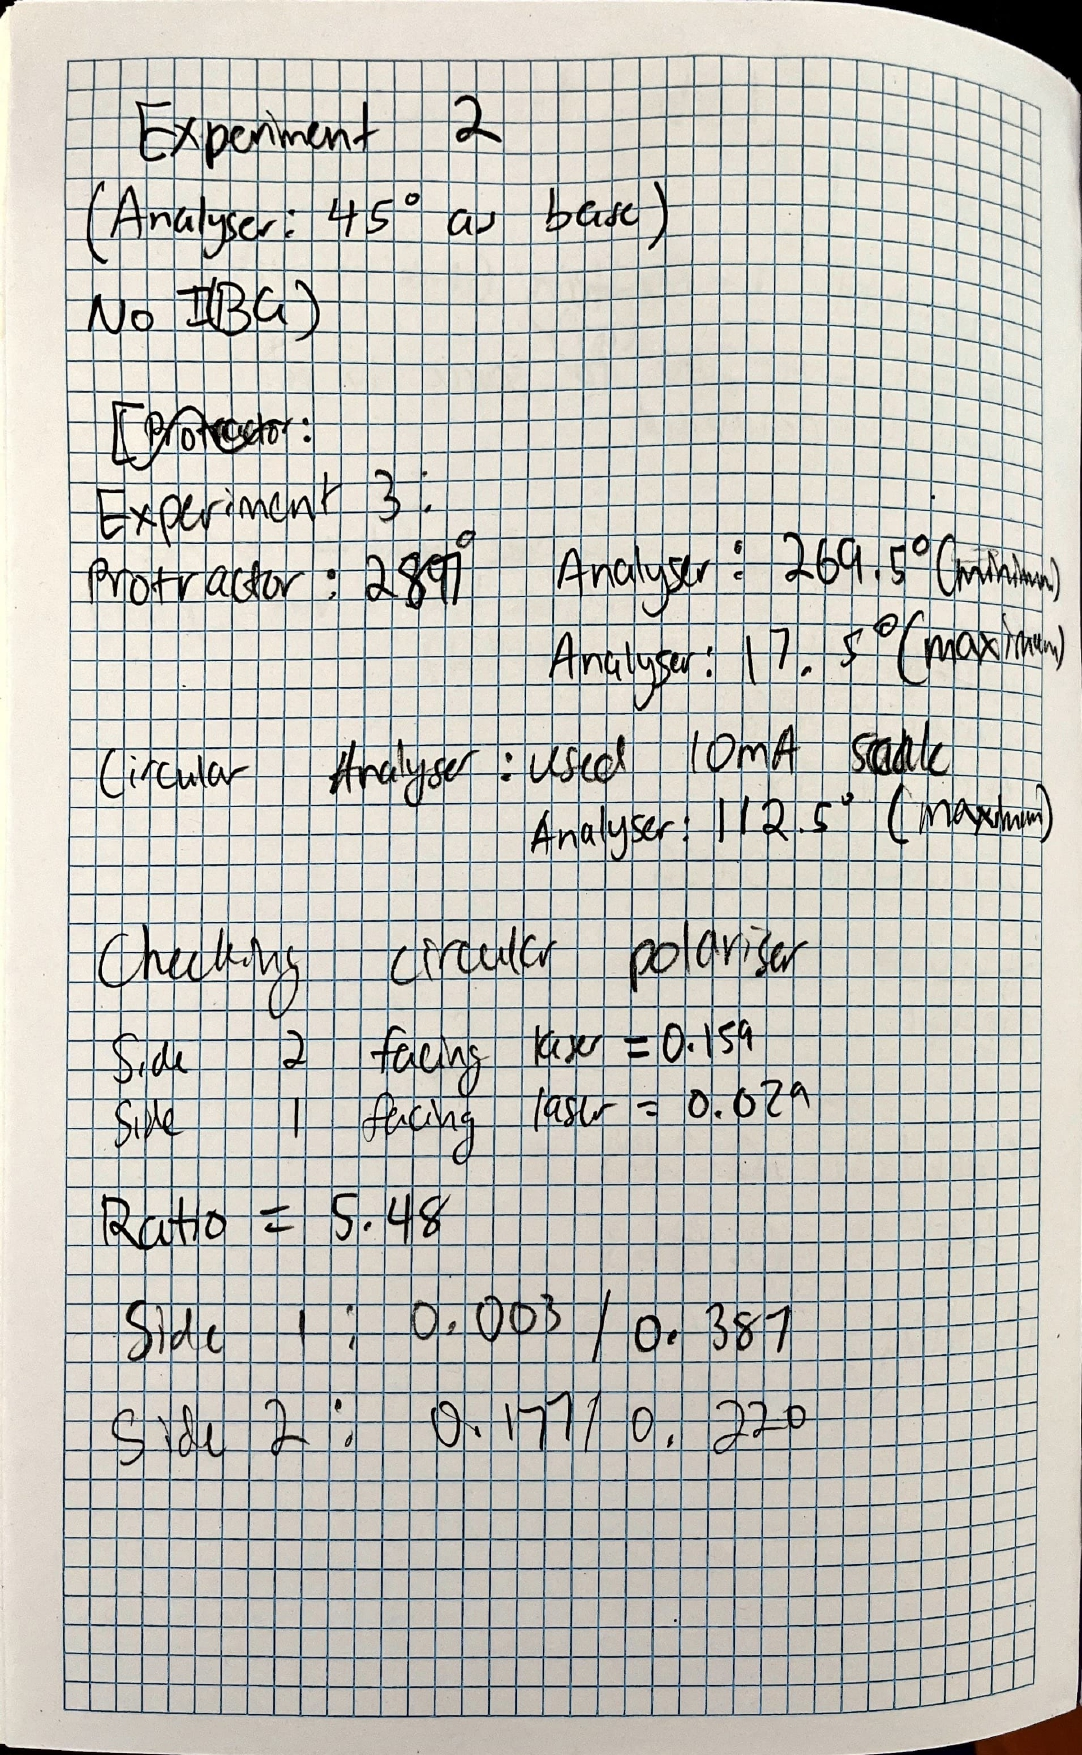
\includegraphics[width=0.8\textwidth]{labbook2.jpg}
\end{figure}

\begin{figure}[H]
    \centering
    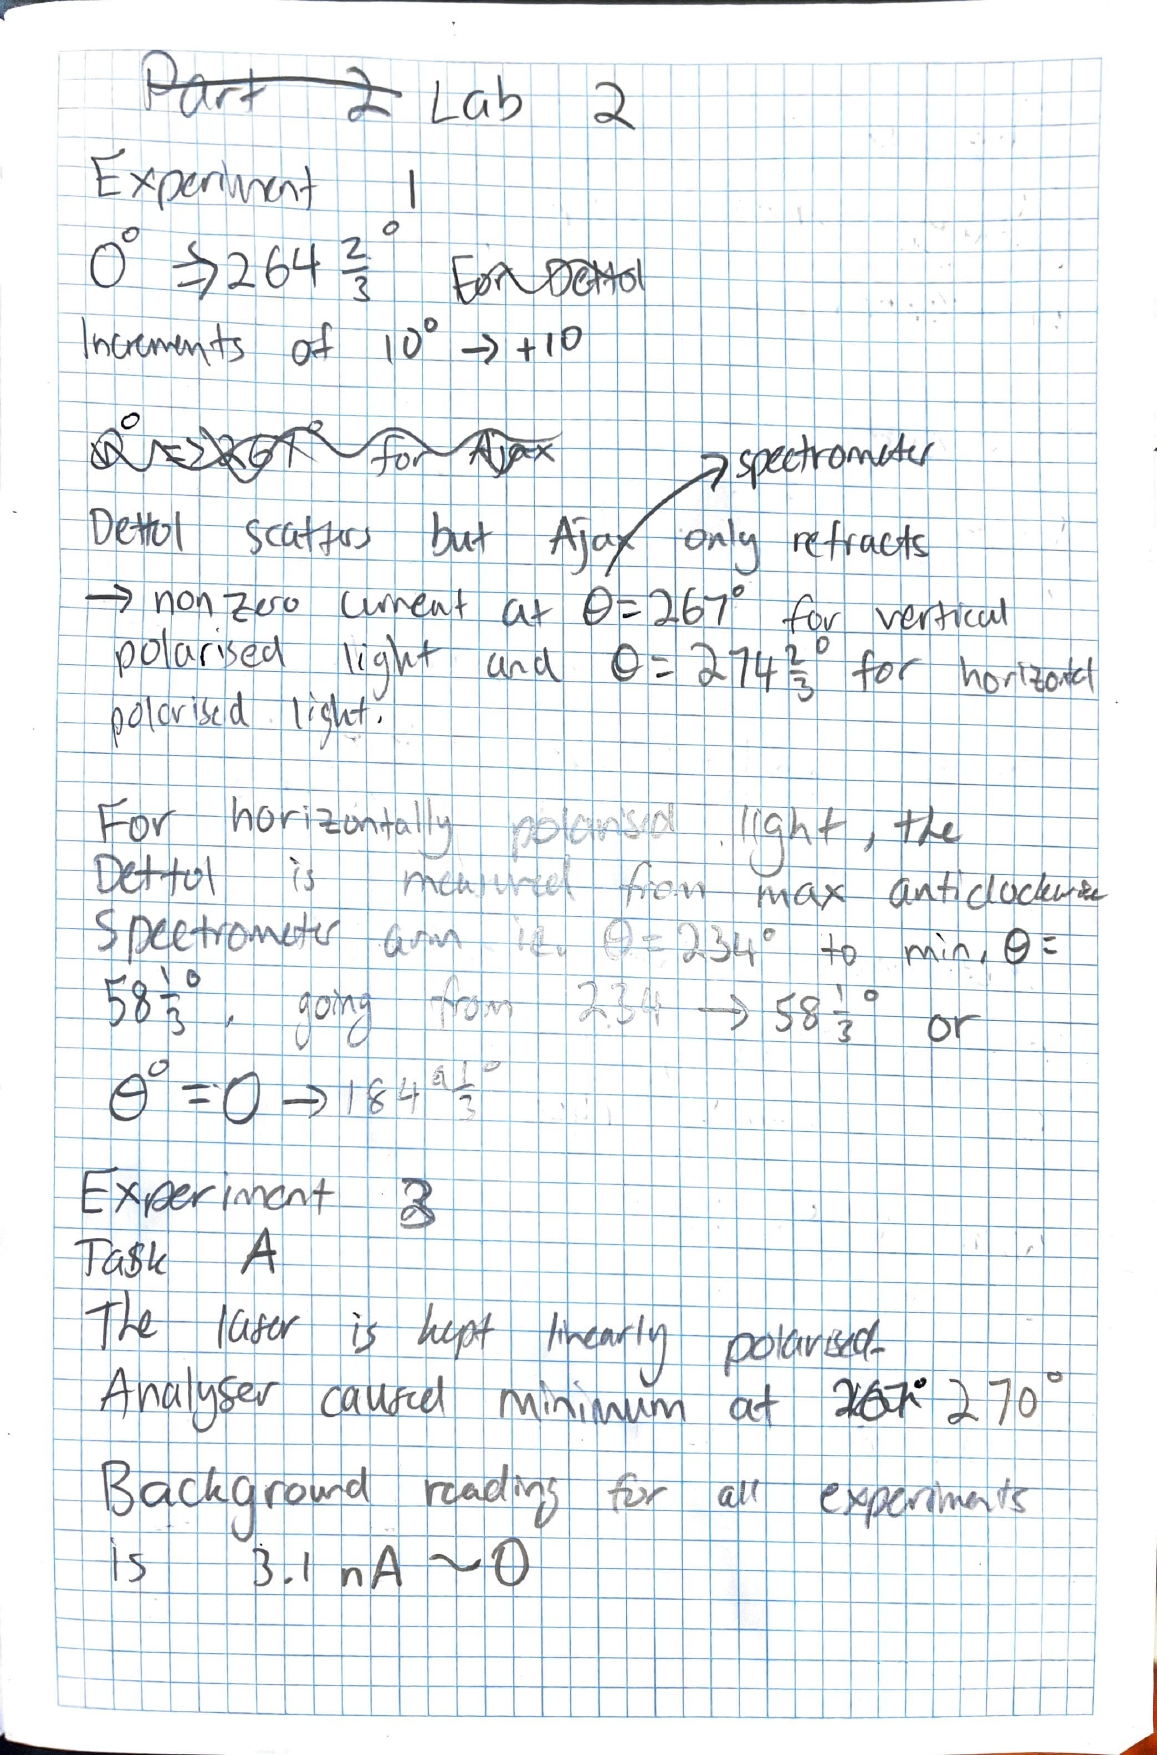
\includegraphics[width=0.8\textwidth]{labbook4.jpg}
\end{figure}

\begin{figure}[H]
    \centering
    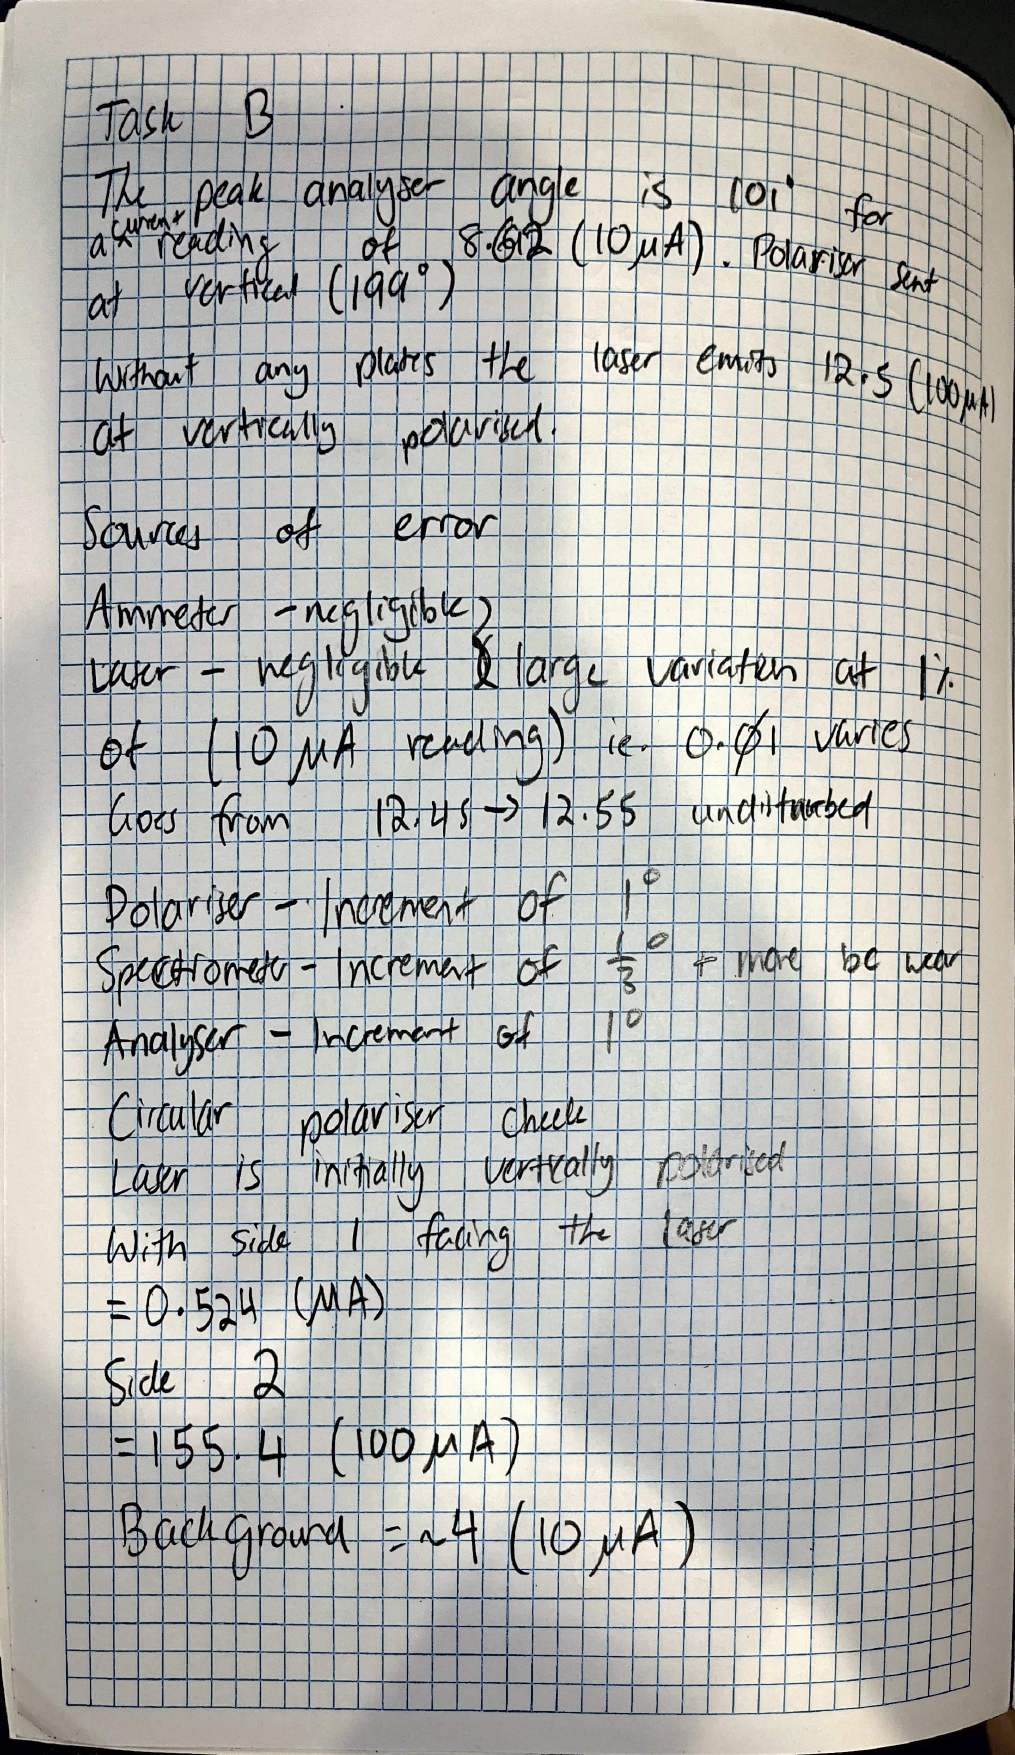
\includegraphics[width=0.8\textwidth]{labbook3.jpg}
\end{figure}

\begin{figure}[H]
    \centering
    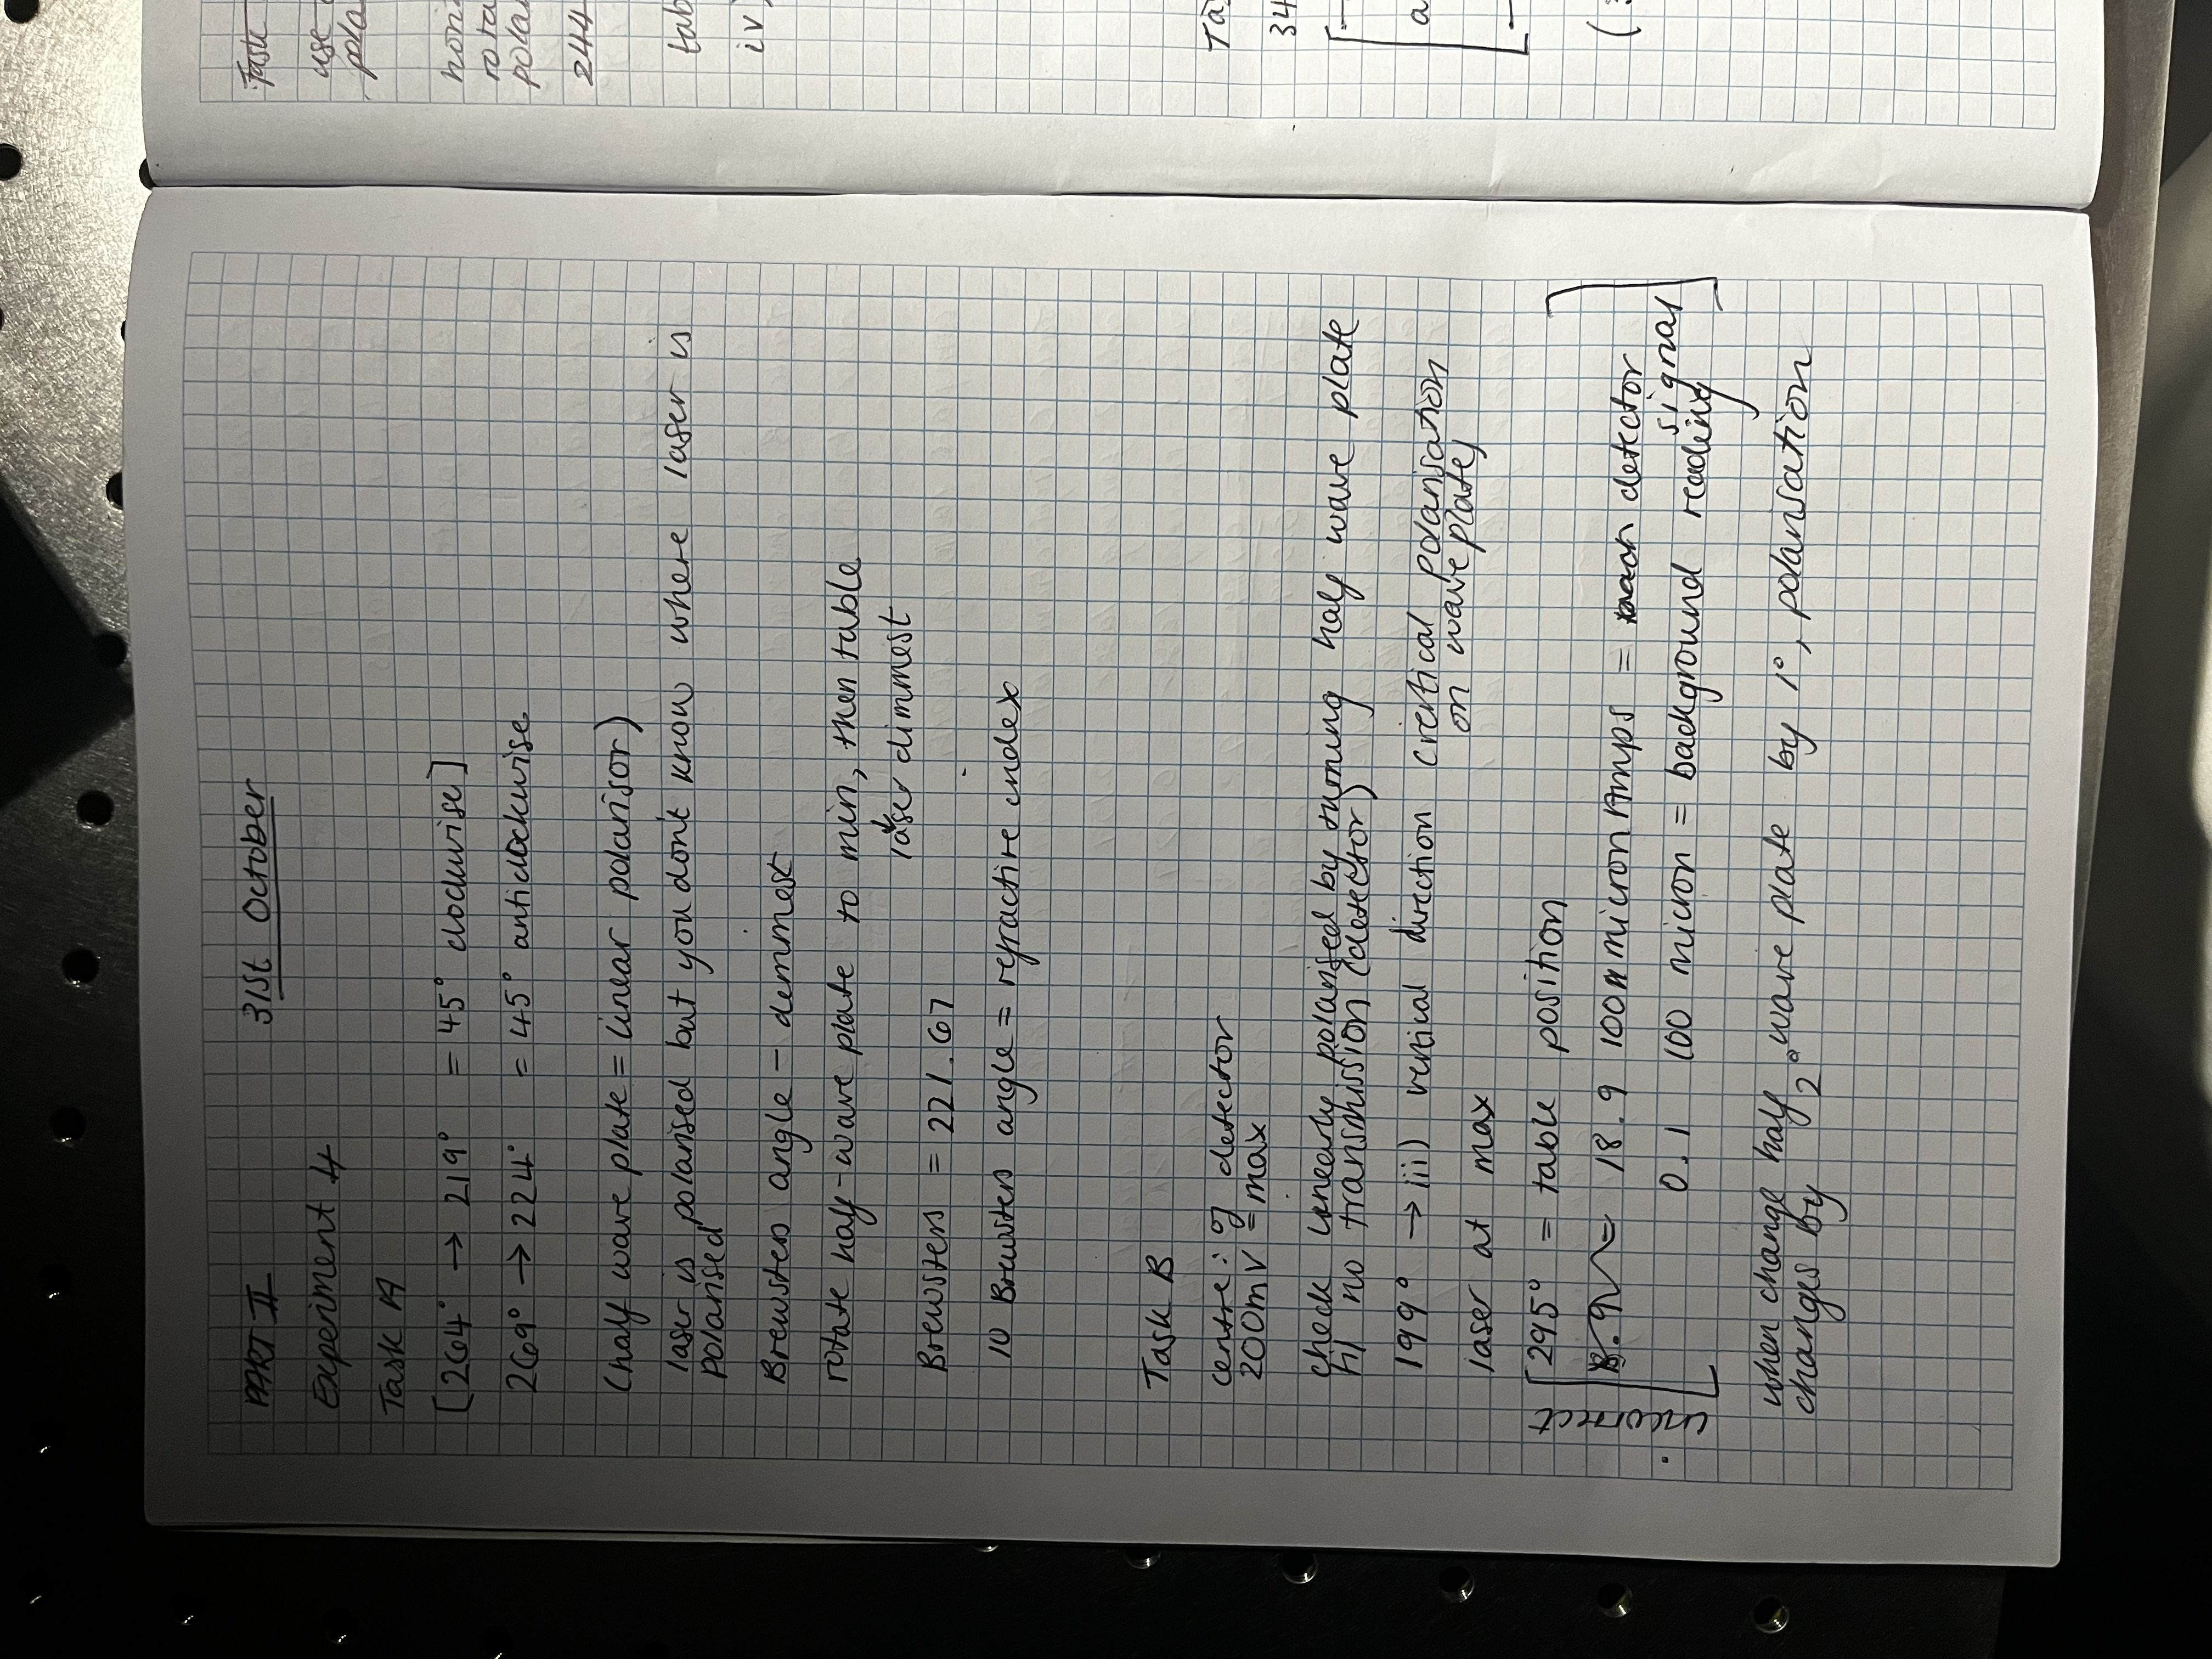
\includegraphics[width=1.2\textwidth,angle=270,origin=c]{labbook8.jpg}
\end{figure}

\begin{figure}[H]
    \centering
    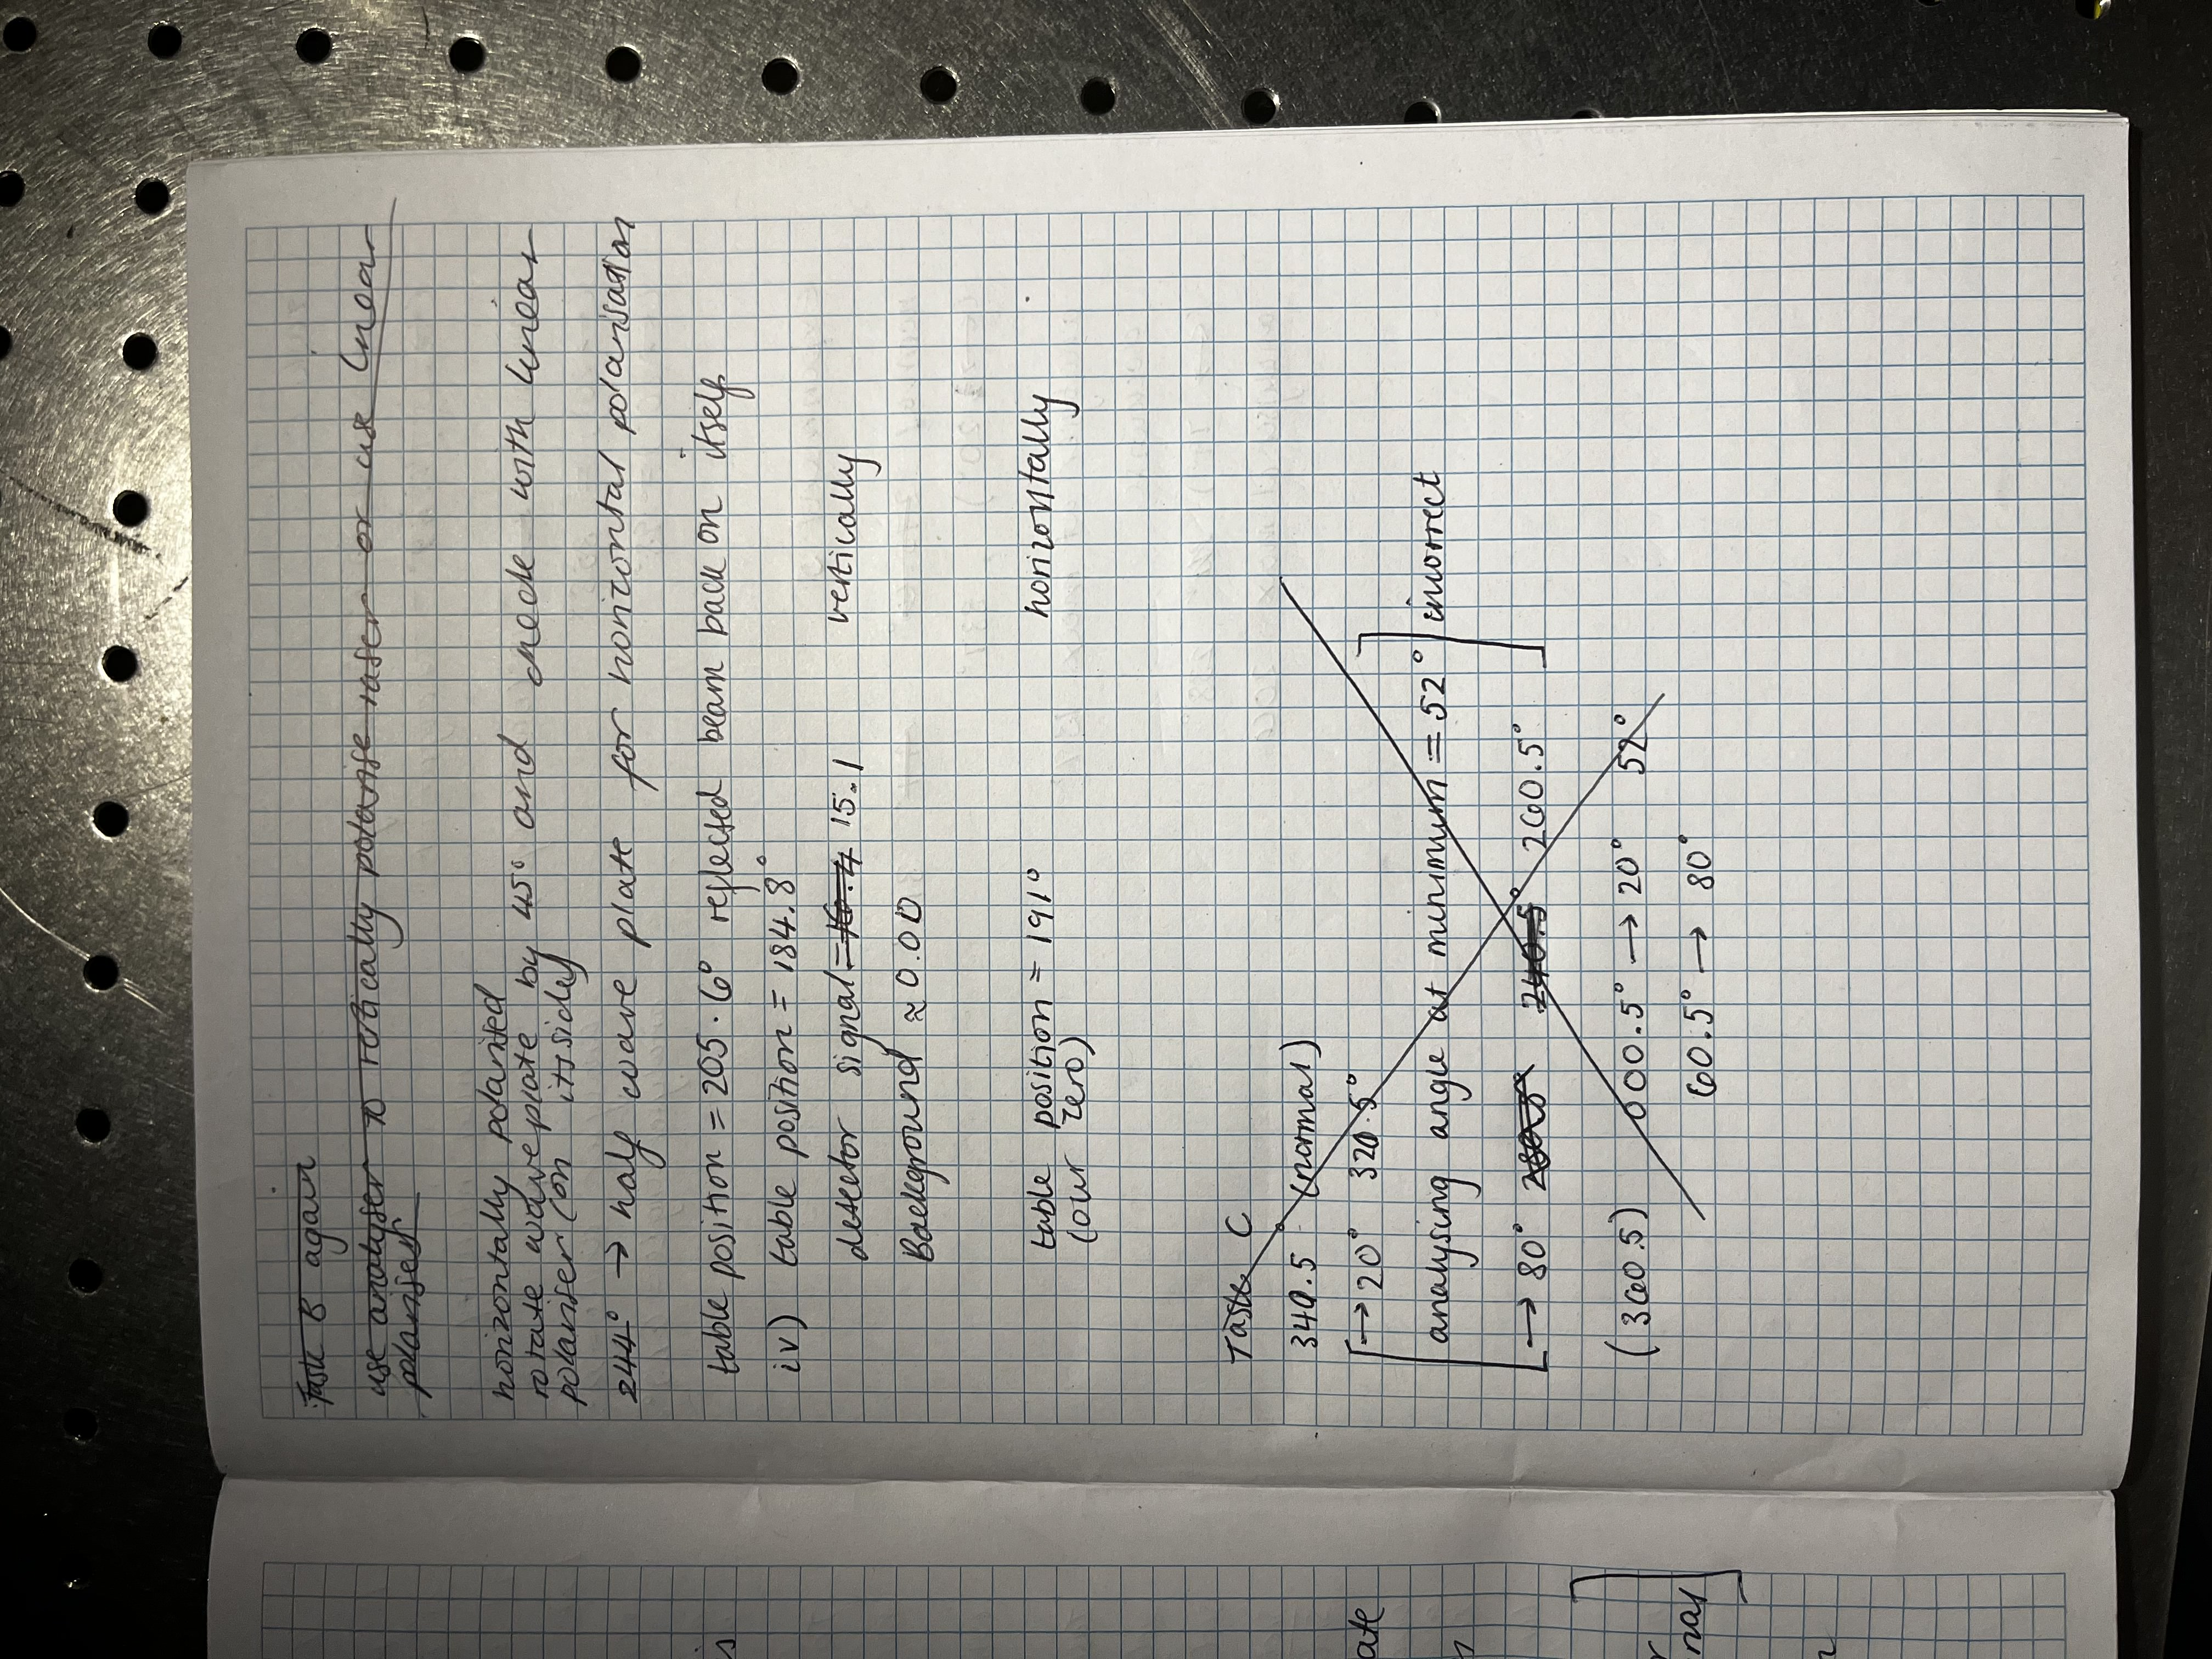
\includegraphics[width=1.2\textwidth,angle=270,origin=c]{labbook9.jpg}
\end{figure}

\subsection{Data Analysis in Python}
\subsubsection{Curve Fitting}

Python was used to create theoretical models to best fit the 
experimental data. First the cosine squared function was defined 
with parameters: $I_0$, theta0 and offset with variable theta. The 
amplitude is given by the initial intensity, $I_0$, the phase shift 
is given by theta0 and the vertical displacement of the funtion 
is given by the parameter offset.

\begin{python}
def curve(theta,I_0,theta0,offset):
    return I_0 * np.cos(np.radians((theta - theta0)))**2 + offset
\end{python}

Using the scipy optimize package, the curve fit function can be 
used which uses a least-squares algorithm to guess the parameters 
that best fits the data input. An example can be seen below,

\begin{python}
x = data['Angle (degrees)']
y = data['Current (micro amps)']

param,covariance = sp.curve_fit(curve,x,y)
\end{python}

The return of the function is of course an array, param, of the best 
fitting parameters.

Rather than plotting the model as a function of the experimental data,
the model was plotted over a a higher resolution of x values to provide 
a smoother curve.

\begin{python}
x_smooth = np.linspace(x.min(),x.max(),1000)
y_smooth = curve(x_smooth,*param)
plt.plot(
    x_smooth,
    y_smooth,
    label=rf'$I_0$={param[0]:.2f}, $\theta_0$ = {param[1]:.2f}, offset = {param[2]:.3f}'
)
\end{python}

\end{document}